\documentclass{beamer}
\usepackage{graphicx}
\usepackage{geometry}
\usepackage{subcaption}
\usepackage{tikz}
\usepackage{booktabs}
\usetikzlibrary{positioning, calc}

\geometry{
  left=1.5cm,
  right=1.5cm,
}

\setbeamerfont{footnote}{size=\tiny}

\title{Chinese Character Recognition:\\Applied to Modern Literature}
\author{Author: Michael Song\\Supervisor: Sibo Cheng\\Second Marker: Pancham Shukla}
\institute{Imperial College London}
\date{\today}

\begin{document}

\begin{frame}
    \titlepage
\end{frame}

\begin{frame}
    \begin{center}
        \Large{Background}
    \end{center}
    \begin{itemize}
        \item Optical Character Recognition (OCR)\footnote{Image source: \href{https://www.edenai.co/post/analyze-easily-document-files-with-ai-optical-character-recognition-ocr}{click here}}: converting images of text into machine-encoded text.
    \end{itemize}
    \begin{figure}
        \centering
        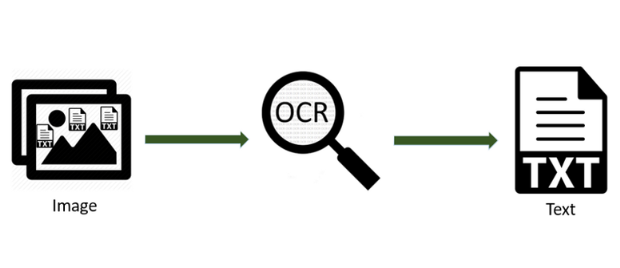
\includegraphics[width=0.75\textwidth]{figures/ocr.png}
    \end{figure}
\end{frame}

\begin{frame}
    \begin{center}
        \Large{Background}
    \end{center}
    \begin{itemize}
        \item Funü Zazhi\footnote{Image source: \href{https://mhdb.mh.sinica.edu.tw/fnzz/image.php?book=1501&page=1}{click here}}: a historical Chinese feminist journal (1915-1931), valuable for research on gender discourse.
    \end{itemize}
    \begin{figure}
        \centering
        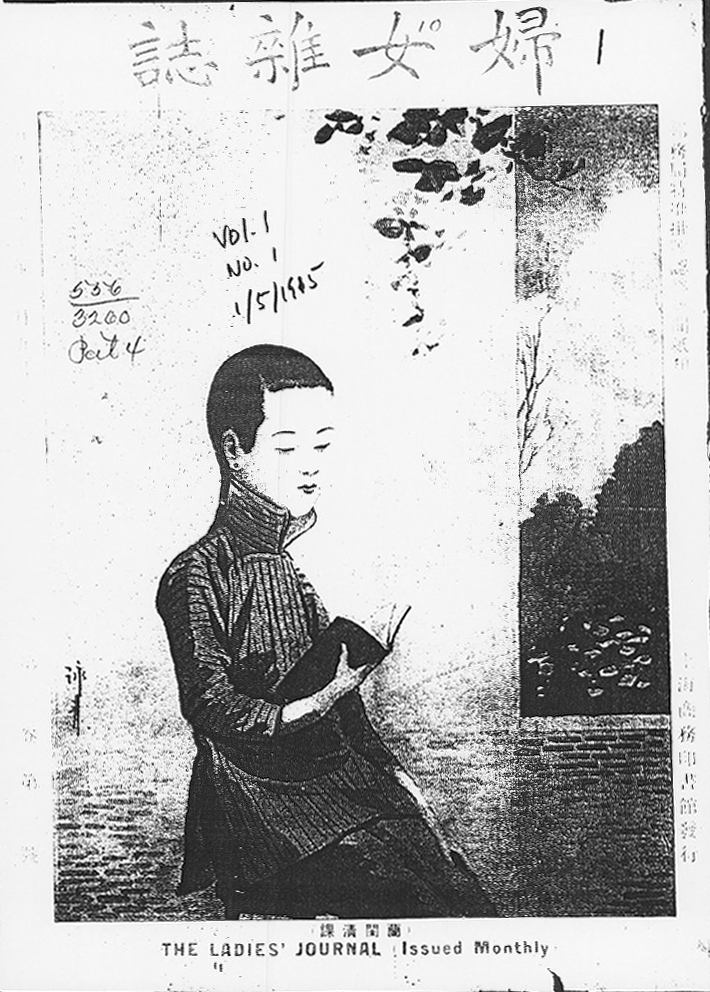
\includegraphics[width=0.4\textwidth]{figures/fnzz.jpg}
    \end{figure}
\end{frame}

\begin{frame}
    \begin{center}
        \Large{Motivation}
    \end{center}
    \begin{itemize}
        \item We want to analyze the content of Funü Zazhi by Natural Language Processing (NLP) using \textbf{computers}.
        \item However, the digital database\footnote{\url{https://mhdb.mh.sinica.edu.tw/fnzz/view.php}} of Funü Zazhi only contains scanned \textbf{images}.
        \item Therefore, we need to convert these images into machine-readable \textbf{text}!
    \end{itemize}
\end{frame}

\begin{frame}
    \begin{center}
        \Large{Challenges}
    \end{center}
    \begin{itemize}
        \item Low resolution characters, diverse text layouts, varying image quality...
    \end{itemize}
    \begin{figure}[htbp]
        \centering
        \begin{subfigure}[b]{0.23\linewidth}
            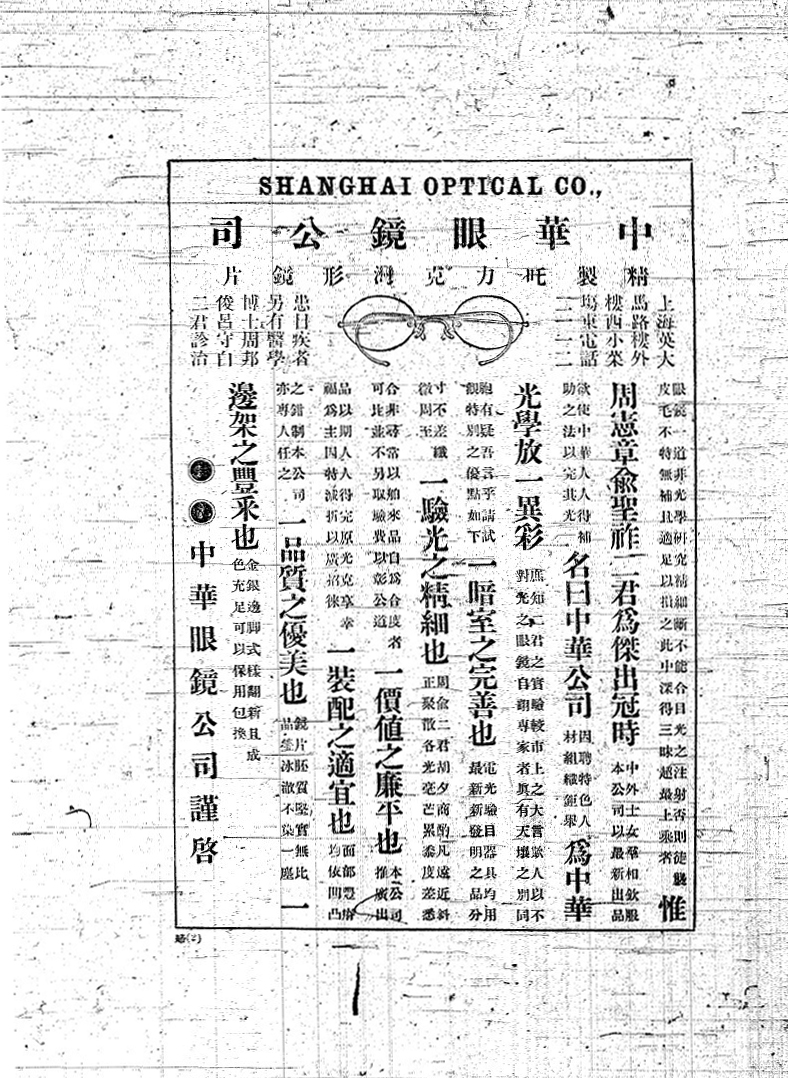
\includegraphics[height=1.3\linewidth]{./figures/fnzz1}
        \end{subfigure}
        \hfill
        \begin{subfigure}[b]{0.23\linewidth}
            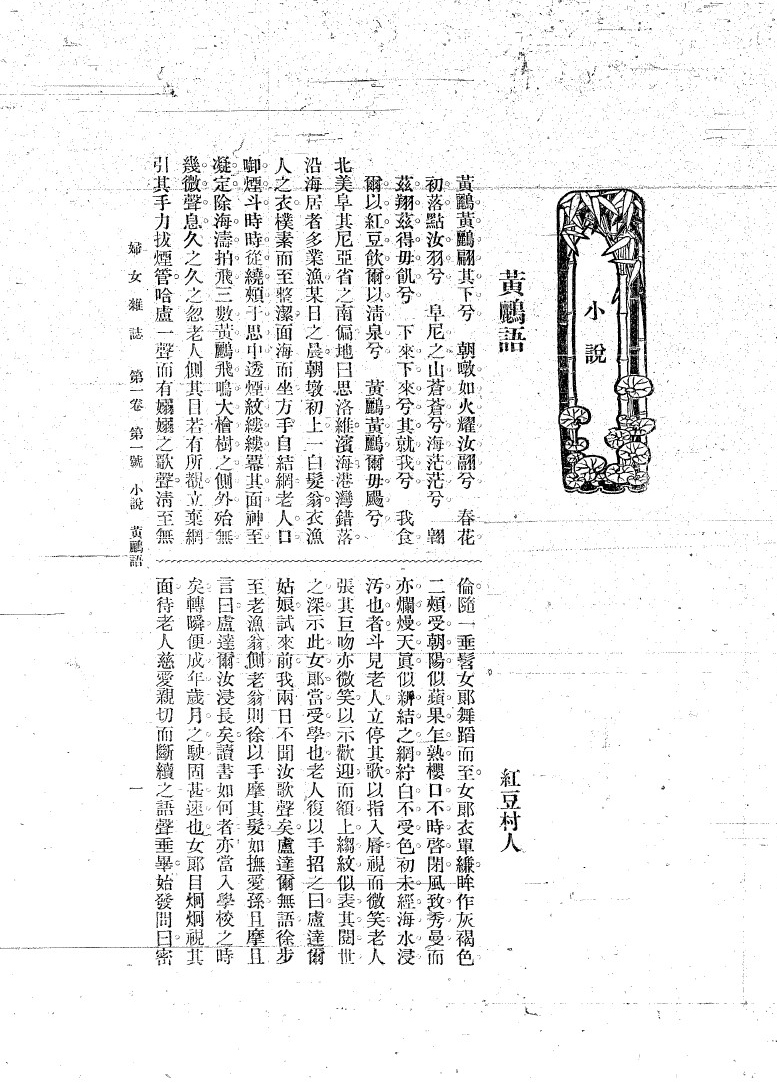
\includegraphics[height=1.3\linewidth]{./figures/fnzz2}
        \end{subfigure}
        \hfill
        \begin{subfigure}[b]{0.23\linewidth}
            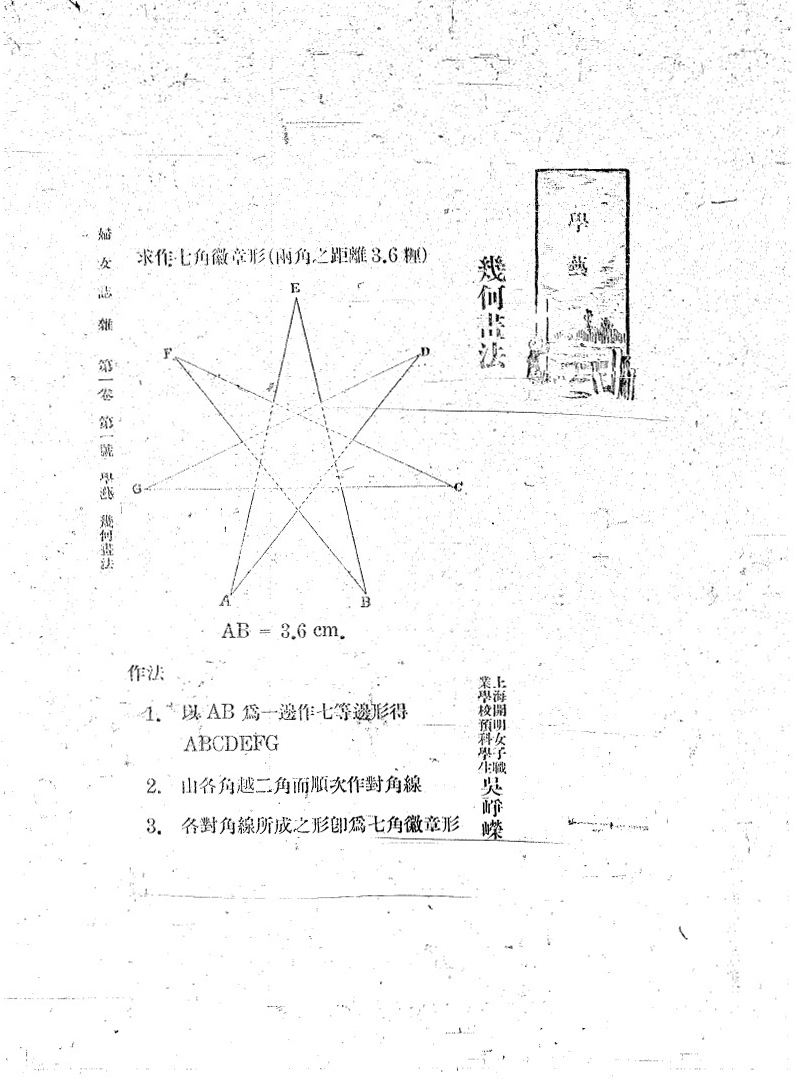
\includegraphics[height=1.3\linewidth]{./figures/fnzz3}
        \end{subfigure}
        \hfill
        \begin{subfigure}[b]{0.23\linewidth}
            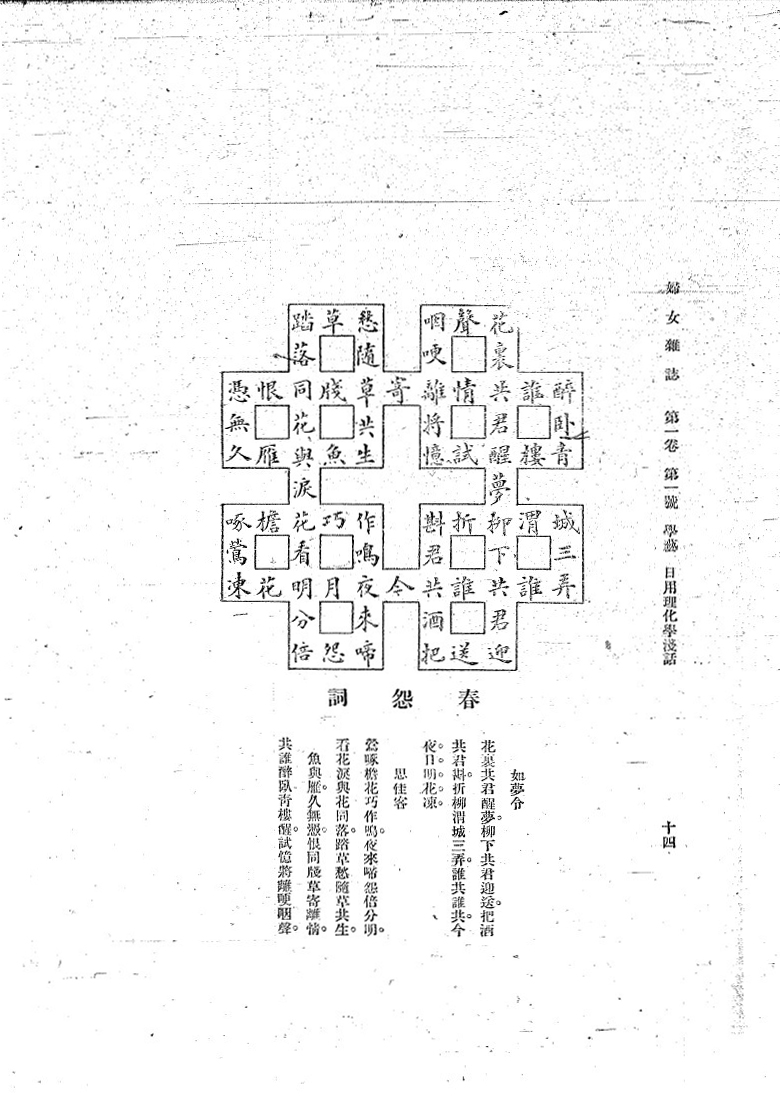
\includegraphics[height=1.3\linewidth]{./figures/fnzz4}
        \end{subfigure}
        \caption{Sample images of Funü Zazhi\footnote{Image source: \href{https://mhdb.mh.sinica.edu.tw/fnzz/view.php}{click here}}}
    \end{figure}
\end{frame}

\begin{frame}
    \begin{center}
        \Large{Challenges}
    \end{center}
    \begin{itemize}
        \item Lack of annotated datasets with \textbf{similar features}.
        \item OCR tools trained on common datasets have poor performance on Funü Zazhi (less than 50\% accuracy!).
    \end{itemize}
    \begin{figure}
        \centering
        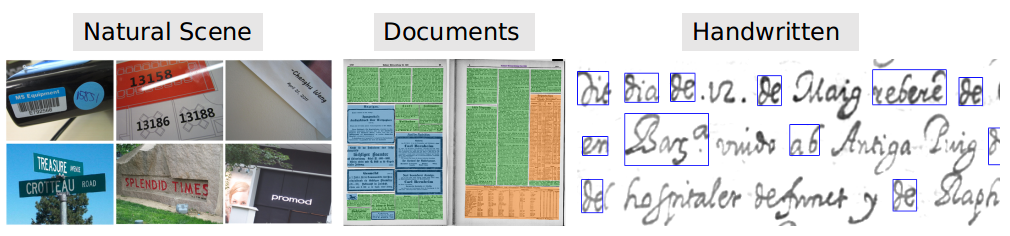
\includegraphics[width=\textwidth]{figures/datasets.png}
        \caption{Common OCR datasets that do not resemble Funü Zazhi\footnote{Image source: \href{https://github.com/xinke-wang/OCRDatasets?tab=readme-ov-file}{click here}}}
    \end{figure}
\end{frame}

\begin{frame}
    \begin{center}
        \Large{Main Goals}
    \end{center}
    \begin{itemize}
        \item Develop an optimized OCR system.
        \item Generate annotated synthetic data to simulate Funü Zazhi images for training.
        \item Perform OCR on 36,101 Funü Zazhi images.
    \end{itemize}
\end{frame}

\begin{frame}
    \begin{center}
        \Large{Related Work}
    \end{center}
    \begin{itemize}
        \item Text Detection: locate text regions in the image.
        \item Text Recognition: convert text region into text.
        \item Two-stage OCR: separate detection and recognition into two models.
        \item End-to-end OCR: combine detection and recognition into a single model.
    \end{itemize}
\end{frame}

\begin{frame}
    \begin{center}
        \Large{Our Approach}
    \end{center}
    \begin{itemize}
        \item Two-stage OCR system.
        \item Special text ordering module for Funü Zazhi.
    \end{itemize}
    \begin{figure}[htbp]
        \centering
        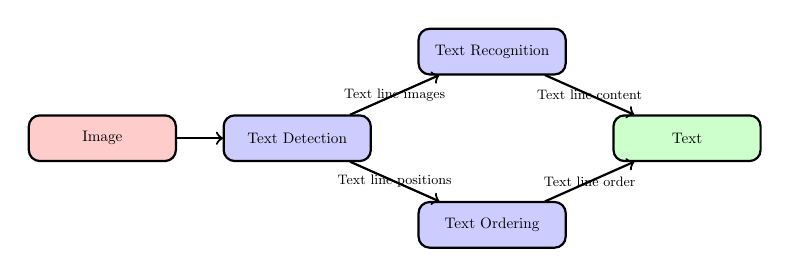
\begin{tikzpicture}[node distance=4.5cm, auto, thick, scale=0.55, transform shape]
            % Define block styles
            \tikzstyle{block} = [rectangle, draw, fill=blue!20, text width=9em, text centered, rounded corners, minimum height=3em]
    
            % Place nodes
            \node [block, fill=red!20] (image) {Image};
            \node [block, right of=image] (text_detection) {Text Detection};
            \node [block, right of=text_detection, yshift=2cm] (text_recognition) {Text Recognition};
            \node [block, right of=text_detection, yshift=-2cm] (text_ordering) {Text Ordering};
            \node [block, fill=green!20, right of=text_ordering, yshift=2cm] (text) {Text};
    
            % Draw connections as arrows
            \draw [->] (image) -- (text_detection);
            \draw [->] (text_detection) -- (text_recognition);
            \draw [->] (text_detection) -- (text_ordering);
            \draw [->] (text_recognition) -- (text);
            \draw [->] (text_ordering) -- (text);
    
            % Add text on the arrows
            \node[align=center] at ($(text_detection)!0.5!(text_recognition)$) {\small Text line images};
            \node[align=center] at ($(text_detection)!0.5!(text_ordering)$) {\small Text line positions};
            \node[align=center] at ($(text_recognition)!0.5!(text)$) {\small Text line content};
            \node[align=center] at ($(text_ordering)!0.5!(text)$) {\small Text line order};
        \end{tikzpicture}
        \caption{Overall structure of the OCR system for Funü Zazhi}
        \label{fig:ocr_system}
    \end{figure}
\end{frame}

\begin{frame}
    \begin{center}
        \Large{Text Detection}
    \end{center}
    \begin{figure}[htbp]
        \centering
        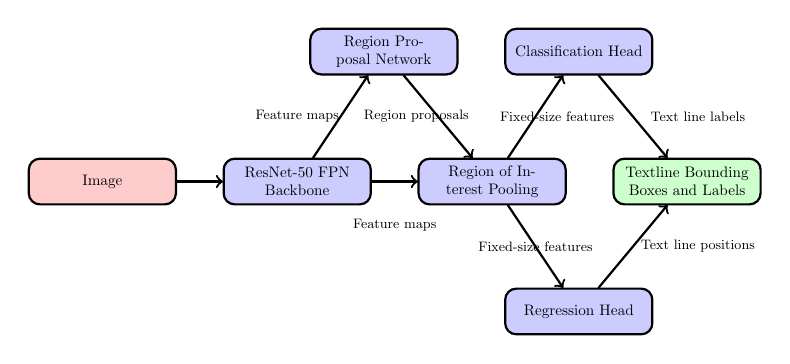
\begin{tikzpicture}[node distance=4.5cm, auto, thick, scale=0.55, transform shape]
            % Define block styles
            \tikzstyle{block} = [rectangle, draw, fill=blue!20, text width=9em, text centered, rounded corners, minimum height=3em]
    
            % Place nodes
            \node [block, fill=red!20] (image) {Image};
            \node [block, right of=image] (backbone) {ResNet-50 FPN Backbone};
            \node [block, right of=backbone, xshift=-2.5cm, yshift=3cm] (rpn) {Region Proposal Network};
            \node [block, right of=backbone] (roi) {Region of Interest Pooling};
            \node [block, right of=roi, xshift=-2.5cm, yshift=3cm] (cla_head) {Classification Head};
            \node [block, right of=roi, xshift=-2.5cm, yshift=-3cm] (reg_head) {Regression Head};
            \node [block, fill=green!20, right of=roi] (output) {Textline Bounding Boxes and Labels};
    
            % Draw connections as arrows
            \draw [->] (image) -- (backbone);
            \draw [->] (backbone) -- (rpn);
            \draw [->] (backbone) -- (roi);
            \draw [->] (rpn) -- (roi);
            \draw [->] (roi) -- (cla_head);
            \draw [->] (roi) -- (reg_head);
            \draw [->] (cla_head) -- (output);
            \draw [->] (reg_head) -- (output);
    
            % Add text on the arrows
            \node[align=center, xshift=-1cm] at ($(backbone)!0.5!(rpn)$) {\small Feature maps};
            \node[align=center, yshift=-1cm] at ($(backbone)!0.5!(roi)$) {\small Feature maps};
            \node[align=center, xshift=-0.5cm] at ($(rpn)!0.5!(roi)$) {\small Region proposals};
            \node[align=center, xshift=0.5cm] at ($(roi)!0.5!(cla_head)$) {\small Fixed-size features};
            \node[align=center] at ($(roi)!0.5!(reg_head)$) {\small Fixed-size features};
            \node[align=center, xshift=1.5cm] at ($(cla_head)!0.5!(output)$) {\small Text line labels};
            \node[align=center, xshift=1.5cm] at ($(reg_head)!0.5!(output)$) {\small Text line positions};
    
        \end{tikzpicture}
        \caption{Faster R-CNN\footnote{\url{https://arxiv.org/pdf/1506.01497}} architecture for text detection}
        \label{fig:faster_rcnn}
    \end{figure}
\end{frame}

\begin{frame}
    \begin{center}
        \Large{Text Recognition}
    \end{center}
    \begin{figure}[htbp]
        \centering
        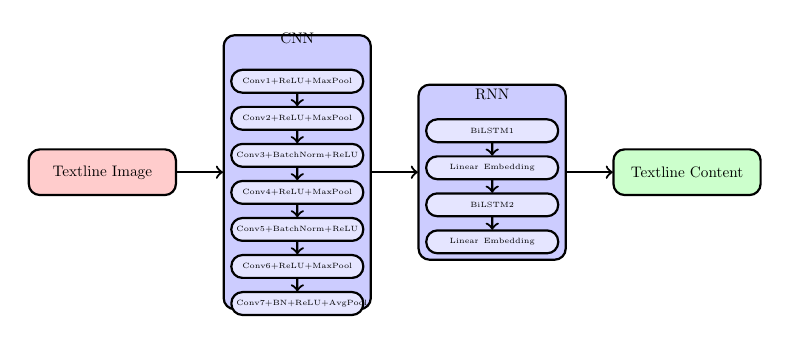
\begin{tikzpicture}[node distance=4.5cm, auto, thick, scale=0.55, transform shape]
            % Define block styles
            \tikzstyle{block} = [rectangle, draw, fill=blue!20, text width=9em, text centered, rounded corners, minimum height=3em]
            \tikzstyle{smallblock} = [rectangle, draw, fill=blue!10, text width=8em, text centered, rounded corners, minimum height=1.5em]
    
            % Place main nodes
            \node [block, fill=red!20] (image) {Textline Image};
            \node [block, right of=image, minimum height=18em] (cnn) {};
            \node [block, right of=cnn, minimum height=11.5em] (rnn) {};
            \node [block, fill=green!20, right of=rnn] (output) {Textline Content};
    
            % Place small blocks inside CNN
            \node [smallblock, below=0.8cm of cnn.north] (conv1) {\tiny Conv1+ReLU+MaxPool};
            \node [smallblock, below=0.3cm of conv1] (conv2) {\tiny Conv2+ReLU+MaxPool};
            \node [smallblock, below=0.3cm of conv2] (conv3) {\tiny Conv3+BatchNorm+ReLU};
            \node [smallblock, below=0.3cm of conv3] (conv4) {\tiny Conv4+ReLU+MaxPool};
            \node [smallblock, below=0.3cm of conv4] (conv5) {\tiny Conv5+BatchNorm+ReLU};
            \node [smallblock, below=0.3cm of conv5] (conv6) {\tiny Conv6+ReLU+MaxPool};
            \node [smallblock, below=0.3cm of conv6] (conv7) {\tiny Conv7+BN+ReLU+AvgPool};
    
            % Place small blocks inside RNN
            \node [smallblock, below=0.8cm of rnn.north] (bilstm1) {\tiny BiLSTM1};
            \node [smallblock, below=0.3cm of bilstm1] (embed1) {\tiny Linear Embedding};
            \node [smallblock, below=0.3cm of embed1] (bilstm2) {\tiny BiLSTM2};
            \node [smallblock, below=0.3cm of bilstm2] (embed2) {\tiny Linear Embedding};
    
            % Draw connections as arrows
            \draw [->] (image) -- (cnn);
            \draw [->] (cnn) -- (rnn);
            \draw [->] (rnn) -- (output);
    
            % Draw connections within CNN
            \draw [->] (conv1) -- (conv2);
            \draw [->] (conv2) -- (conv3);
            \draw [->] (conv3) -- (conv4);
            \draw [->] (conv4) -- (conv5);
            \draw [->] (conv5) -- (conv6);
            \draw [->] (conv6) -- (conv7);
    
            % Draw connections within RNN
            \draw [->] (bilstm1) -- (embed1);
            \draw [->] (embed1) -- (bilstm2);
            \draw [->] (bilstm2) -- (embed2);
    
            % Add text on the arrows
            \node[align=center, yshift=3.1cm] at (cnn) {CNN};
            \node[align=center, yshift=1.8cm] at (rnn) {RNN};
    
        \end{tikzpicture}
        \caption{CRNN\footnote{\url{https://arxiv.org/pdf/1507.05717}} architecture for text recognition}
        \label{fig:crnn}
    \end{figure}
\end{frame}

\begin{frame}
    \begin{center}
        \Large{Text Ordering}
    \end{center}
    \begin{itemize}
        \item By default, the detected text lines are ordered by their confidence scores, not the actual \textbf{reading order}.
        \item We need to reorder the text lines to make the whole text readable.
        \item The text ordering module works based on text line \textbf{positions} and \textbf{labels} (vertical/horizontal) given by the text detection model.
    \end{itemize}
\end{frame}

\begin{frame}
    \begin{center}
        \Large{Text Ordering}
    \end{center}
    \begin{itemize}
        \item Around 80\% of the Funü Zazhi images are in a specific layout, we call it L1.
        \item Other images have different layouts, we call them L2.
        \item The algorithm first distinguishes between L1 and L2, by counting the number of \textbf{vertical} text lines in the upper and lower parts of the image respectively.
    \end{itemize}
    \begin{figure}[htbp]
        \centering
        \begin{subfigure}[b]{0.23\linewidth}
            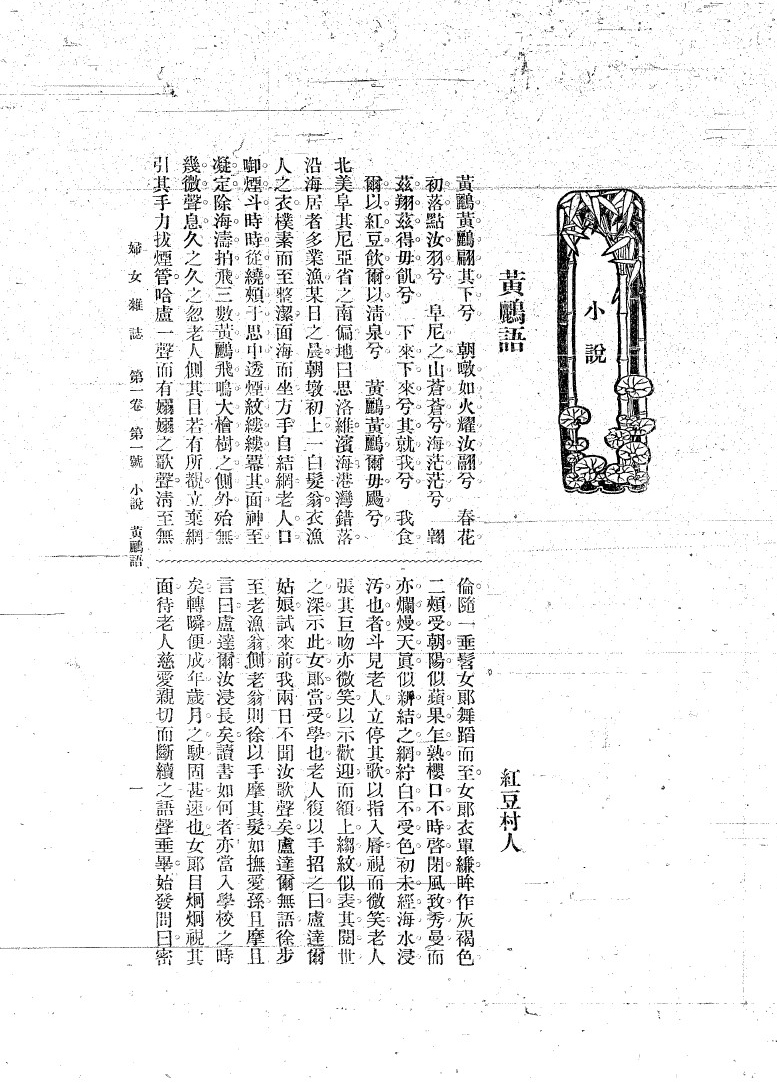
\includegraphics[height=1.3\linewidth]{./figures/fnzz2}
        \end{subfigure}
        \hfill
        \begin{subfigure}[b]{0.23\linewidth}
            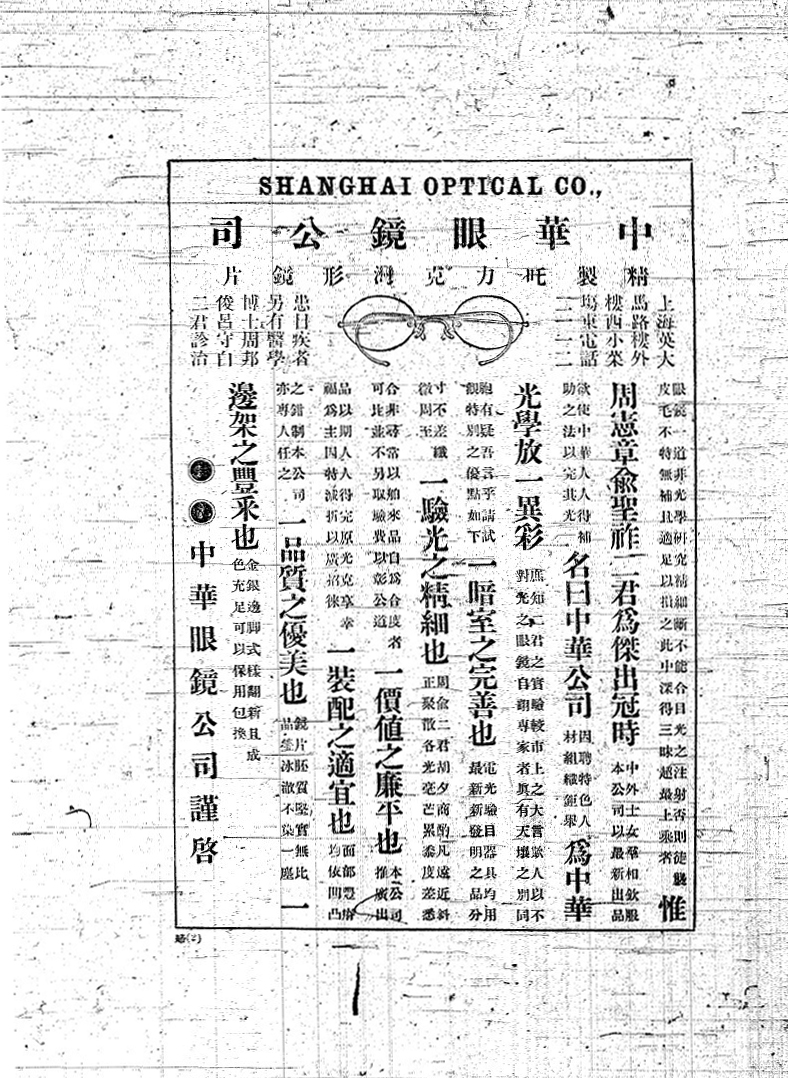
\includegraphics[height=1.3\linewidth]{./figures/fnzz1}
        \end{subfigure}
        \hfill
        \begin{subfigure}[b]{0.23\linewidth}
            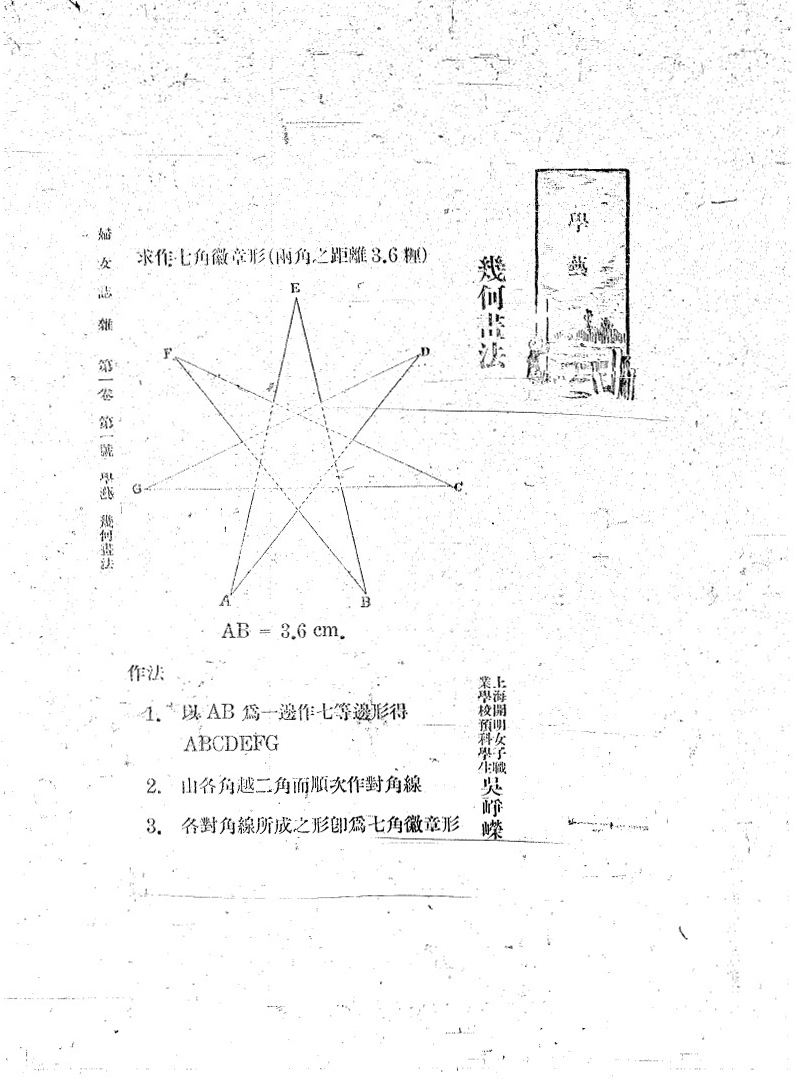
\includegraphics[height=1.3\linewidth]{./figures/fnzz3}
        \end{subfigure}
        \hfill
        \begin{subfigure}[b]{0.23\linewidth}
            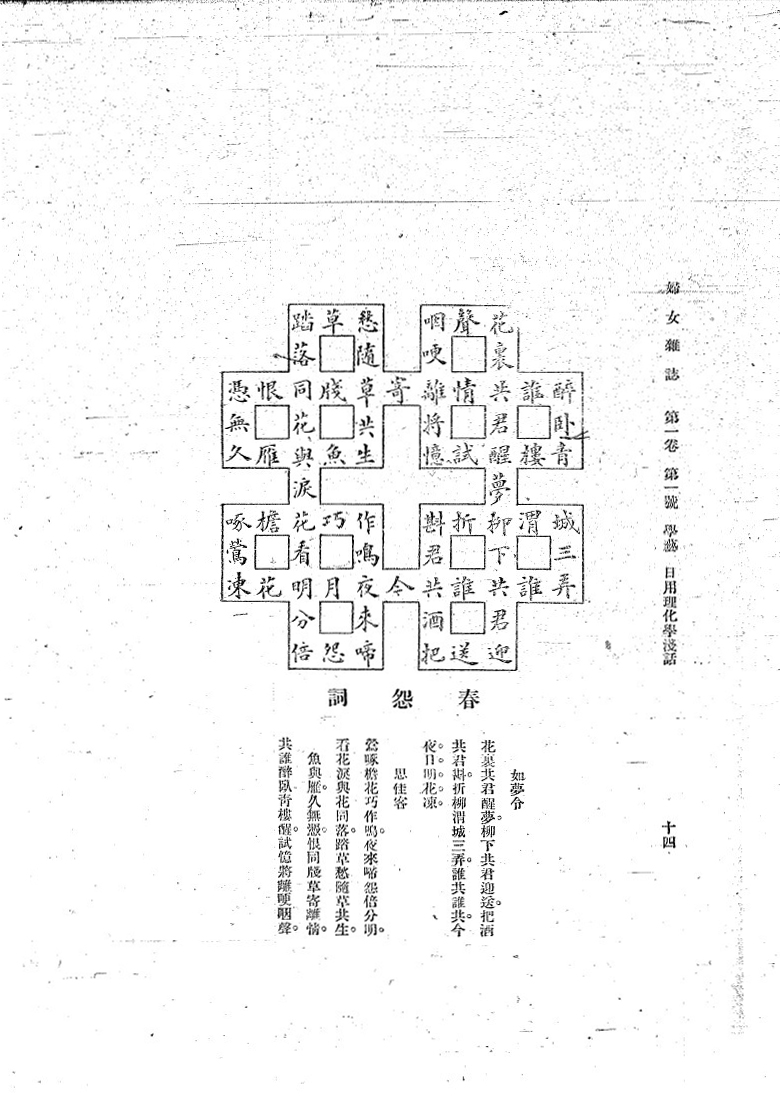
\includegraphics[height=1.3\linewidth]{./figures/fnzz4}
        \end{subfigure}
        \caption{We regard the left image as L1 and other images as L2}
    \end{figure}
\end{frame}

\begin{frame}
    \begin{center}
        \Large{Text Ordering}
    \end{center}
    \begin{itemize}
        \item For L1, the text reading rule is clear.
        \item The algorithm orders the text lines in the upper part and lower part separately, then combines them.
    \end{itemize}
    \begin{figure}
        \centering
        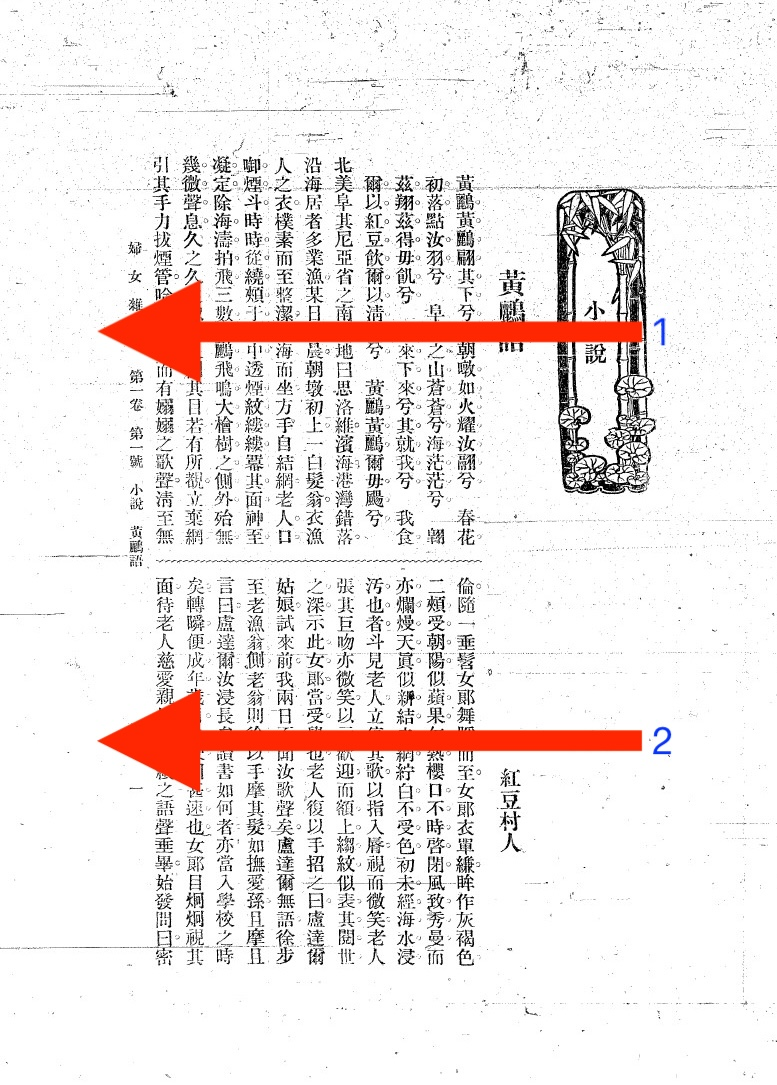
\includegraphics[width=0.35\textwidth]{figures/fnzz2_order.jpeg}
    \end{figure}
\end{frame}

\begin{frame}
    \begin{center}
        \Large{Text Ordering}
    \end{center}
    \begin{itemize}
        \item For L2, the text reading rules are diverse.
        \item But in general, vertical lines are read from right to left, and horizontal lines are read from top to bottom.
        \item The algorithm orders the vertical text lines and horizontal text lines separately, then combines them.
    \end{itemize}
    \begin{figure}
        \begin{subfigure}[b]{0.3\linewidth}
            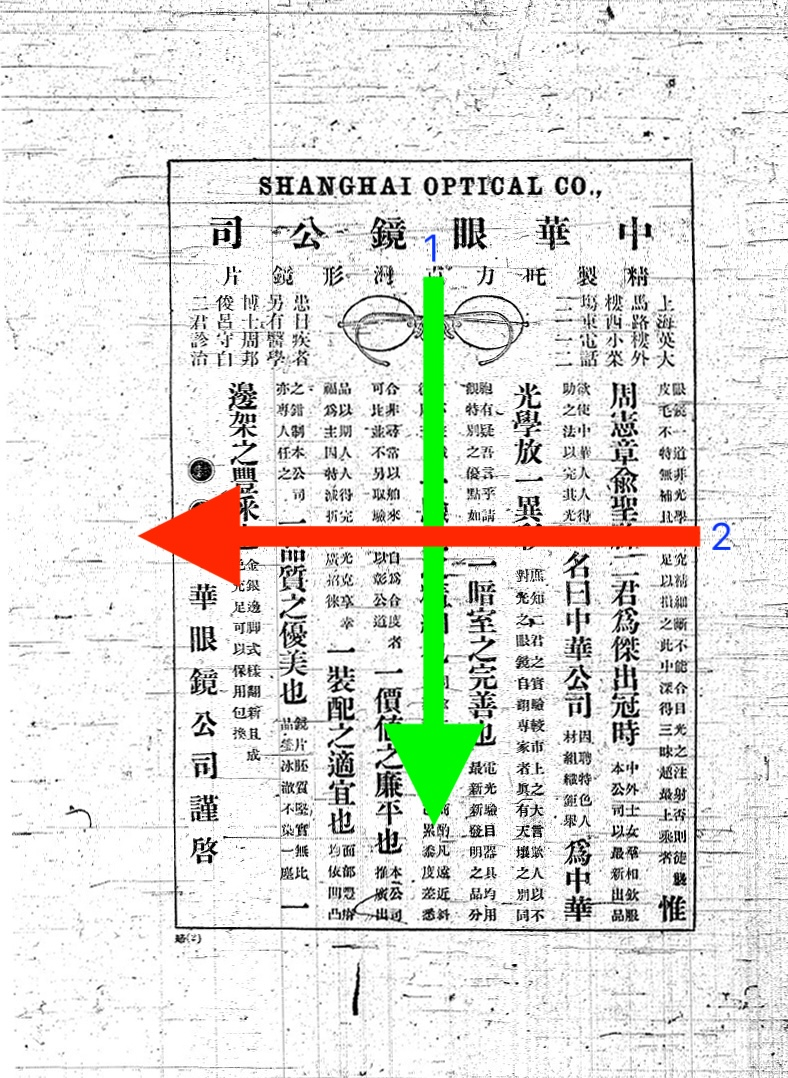
\includegraphics[height=1.3\linewidth]{./figures/fnzz1_order.jpeg}
        \end{subfigure}
        \hspace{1cm}
        \begin{subfigure}[b]{0.3\linewidth}
            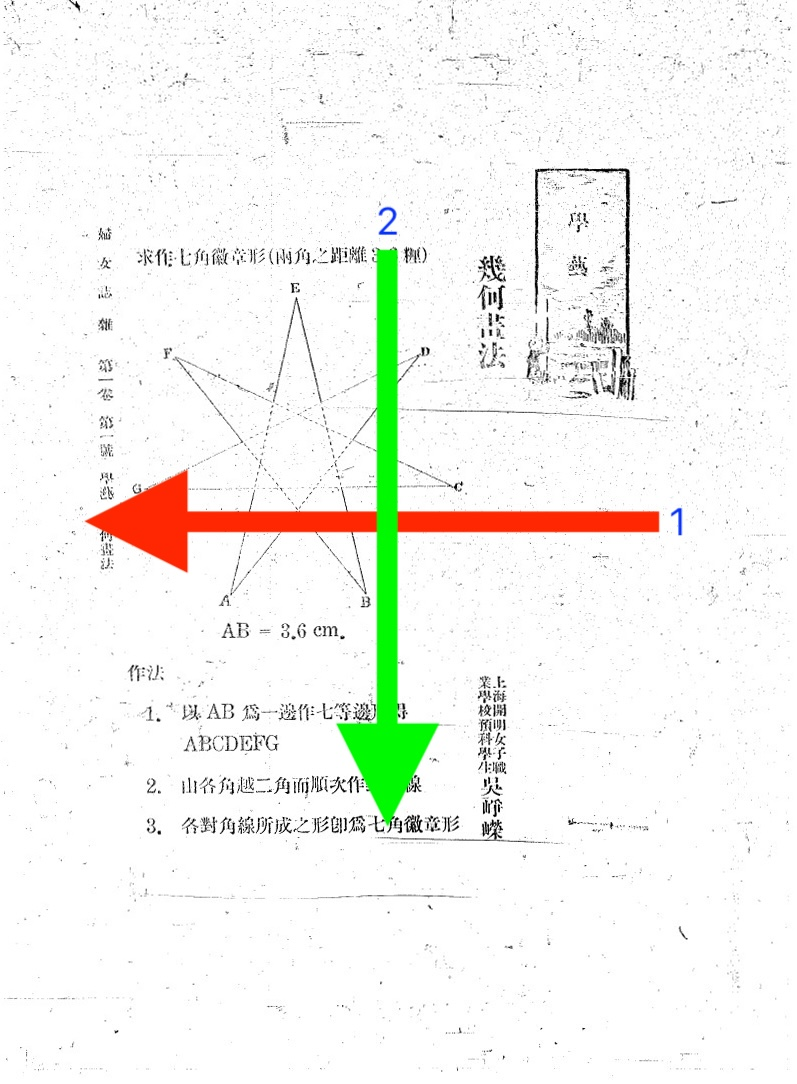
\includegraphics[height=1.3\linewidth]{./figures/fnzz3_order.jpeg}
        \end{subfigure}
    \end{figure}
\end{frame}

\begin{frame}
    \begin{center}
        \Large{Text Ordering}
    \end{center}
    \begin{itemize}
        \item \textbf{Pros}: simple and effective. The major layout L1 can be ordered accurately, while the minor but diverse layout L2 is ordered by a general rule to prevent overfitting.
        \item \textbf{Cons}: need hyperparameters to distinguish L1 and L2, and the general rule may not be accurate for all images.
    \end{itemize}
\end{frame}

\begin{frame}
    \begin{center}
        \Large{Synthetic Data Generation}
    \end{center}
    \begin{itemize}
        \item We generate two types of synthetic data to train the text detection and recognition models respectively.
        \item The synthetic data simulates images of Funü Zazhi, with diverse text layouts and varying image quality.
        \item The synthetic data is generated \textbf{continuously} during the training process.
    \end{itemize}
\end{frame}

\begin{frame}
    \begin{center}
        \Large{Synthetic Data: Basic Units}
    \end{center}
    \begin{itemize}
        \item We select 6,000 most frequent Chinese characters\footnote{\url{https://lingua.mtsu.edu/chinese-computing/statistics/}} as the basic units in the synthetic data.
        \item We use 12 fonts that are commonly used in Funü Zazhi to render each character.
        \item Different characters of a same font form a \textbf{text line}.
    \end{itemize}
    \begin{figure}[htbp]
        \centering
        \begin{subfigure}[b]{0.1\linewidth}
            
\includegraphics[width=\linewidth]{./figures/fonts/642_0.jpg}
            \label{fig:fonts1}
        \end{subfigure}
        \hfill
        \begin{subfigure}[b]{0.1\linewidth}
            
\includegraphics[width=\linewidth]{./figures/fonts/642_1.jpg}
            \label{fig:fonts2}
        \end{subfigure}
        \hfill
        \begin{subfigure}[b]{0.1\linewidth}
            
\includegraphics[width=\linewidth]{./figures/fonts/642_2.jpg}
            \label{fig:fonts3}
        \end{subfigure}
        \hfill
        \begin{subfigure}[b]{0.1\linewidth}
            
\includegraphics[width=\linewidth]{./figures/fonts/642_3.jpg}
            \label{fig:fonts4}
        \end{subfigure}
        \hfill
        \begin{subfigure}[b]{0.1\linewidth}
            
\includegraphics[width=\linewidth]{./figures/fonts/642_4.jpg}
            \label{fig:fonts5}
        \end{subfigure}
        \hfill
        \begin{subfigure}[b]{0.1\linewidth}
            
\includegraphics[width=\linewidth]{./figures/fonts/642_5.jpg}
            \label{fig:fonts6}
        \end{subfigure}
    
        \begin{subfigure}[b]{0.1\linewidth}
            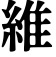
\includegraphics[width=\linewidth]{./figures/fonts/642_6.jpg}
            \label{fig:fonts7}
        \end{subfigure}
        \hfill
        \begin{subfigure}[b]{0.1\linewidth}
            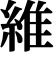
\includegraphics[width=\linewidth]{./figures/fonts/642_7.jpg}
            \label{fig:fonts8}
        \end{subfigure}
        \hfill
        \begin{subfigure}[b]{0.1\linewidth}
            
\includegraphics[width=\linewidth]{./figures/fonts/642_8.jpg}
            \label{fig:fonts9}
        \end{subfigure}
        \hfill
        \begin{subfigure}[b]{0.1\linewidth}
            
\includegraphics[width=\linewidth]{./figures/fonts/642_9.jpg}
            \label{fig:fonts10}
        \end{subfigure}
        \hfill
        \begin{subfigure}[b]{0.1\linewidth}
            
\includegraphics[width=\linewidth]{./figures/fonts/642_10.jpg}
            \label{fig:fonts11}
        \end{subfigure}
        \hfill
        \begin{subfigure}[b]{0.1\linewidth}
            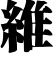
\includegraphics[width=\linewidth]{./figures/fonts/642_11.jpg}
            \label{fig:fonts12}
        \end{subfigure}
        \caption{12 font styles of a specific traditional Chinese character}
        \label{fig:fonts}
    \end{figure}
\end{frame}

\begin{frame}
    \begin{center}
        \Large{Synthetic Data for Detection}
    \end{center}
    \begin{itemize}
        \item Simulate both L1 and L2 layouts.
        \item For L1, divide the image into two parts, and place \textbf{vertical} text lines in each part.
        \item Random noises and \textbf{non-text elements}\footnote{From Icons-50 dataset: \url{https://arxiv.org/abs/1807.01697}} are added to the images to simulate various backgrounds.
    \end{itemize}
    \begin{figure}
        \centering
        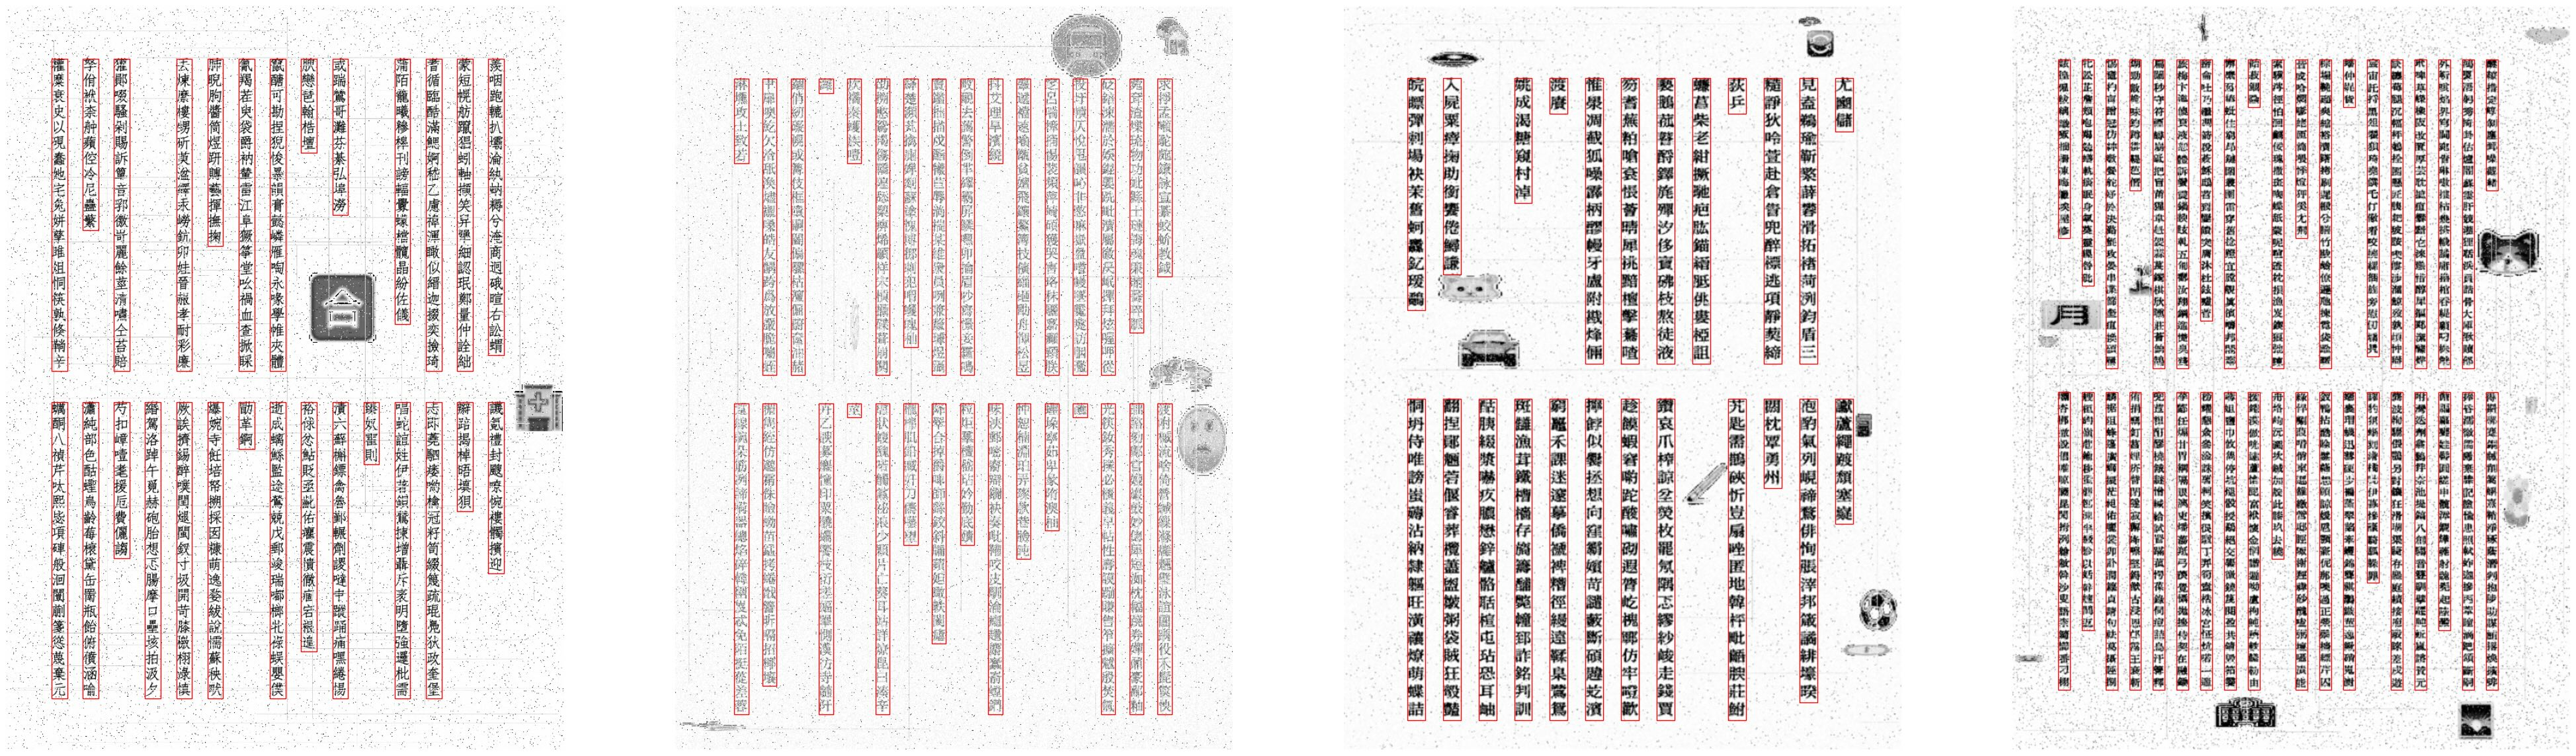
\includegraphics[width=\textwidth]{figures/synthetic_det1.jpeg}
        \caption{Synthetic images for detection with layout L1}
    \end{figure}
\end{frame}

\begin{frame}
    \begin{center}
        \Large{Synthetic Data for Detection}
    \end{center}
    \begin{itemize}
        \item For L2, randomly place both \textbf{vertical} and \textbf{horizontal} text lines in the image.
        \item Each \textbf{text line} uses a random typeface and font size. In L1, the font size and typeface are fixed for each \textbf{image}.
    \end{itemize}
    \begin{figure}
        \centering
        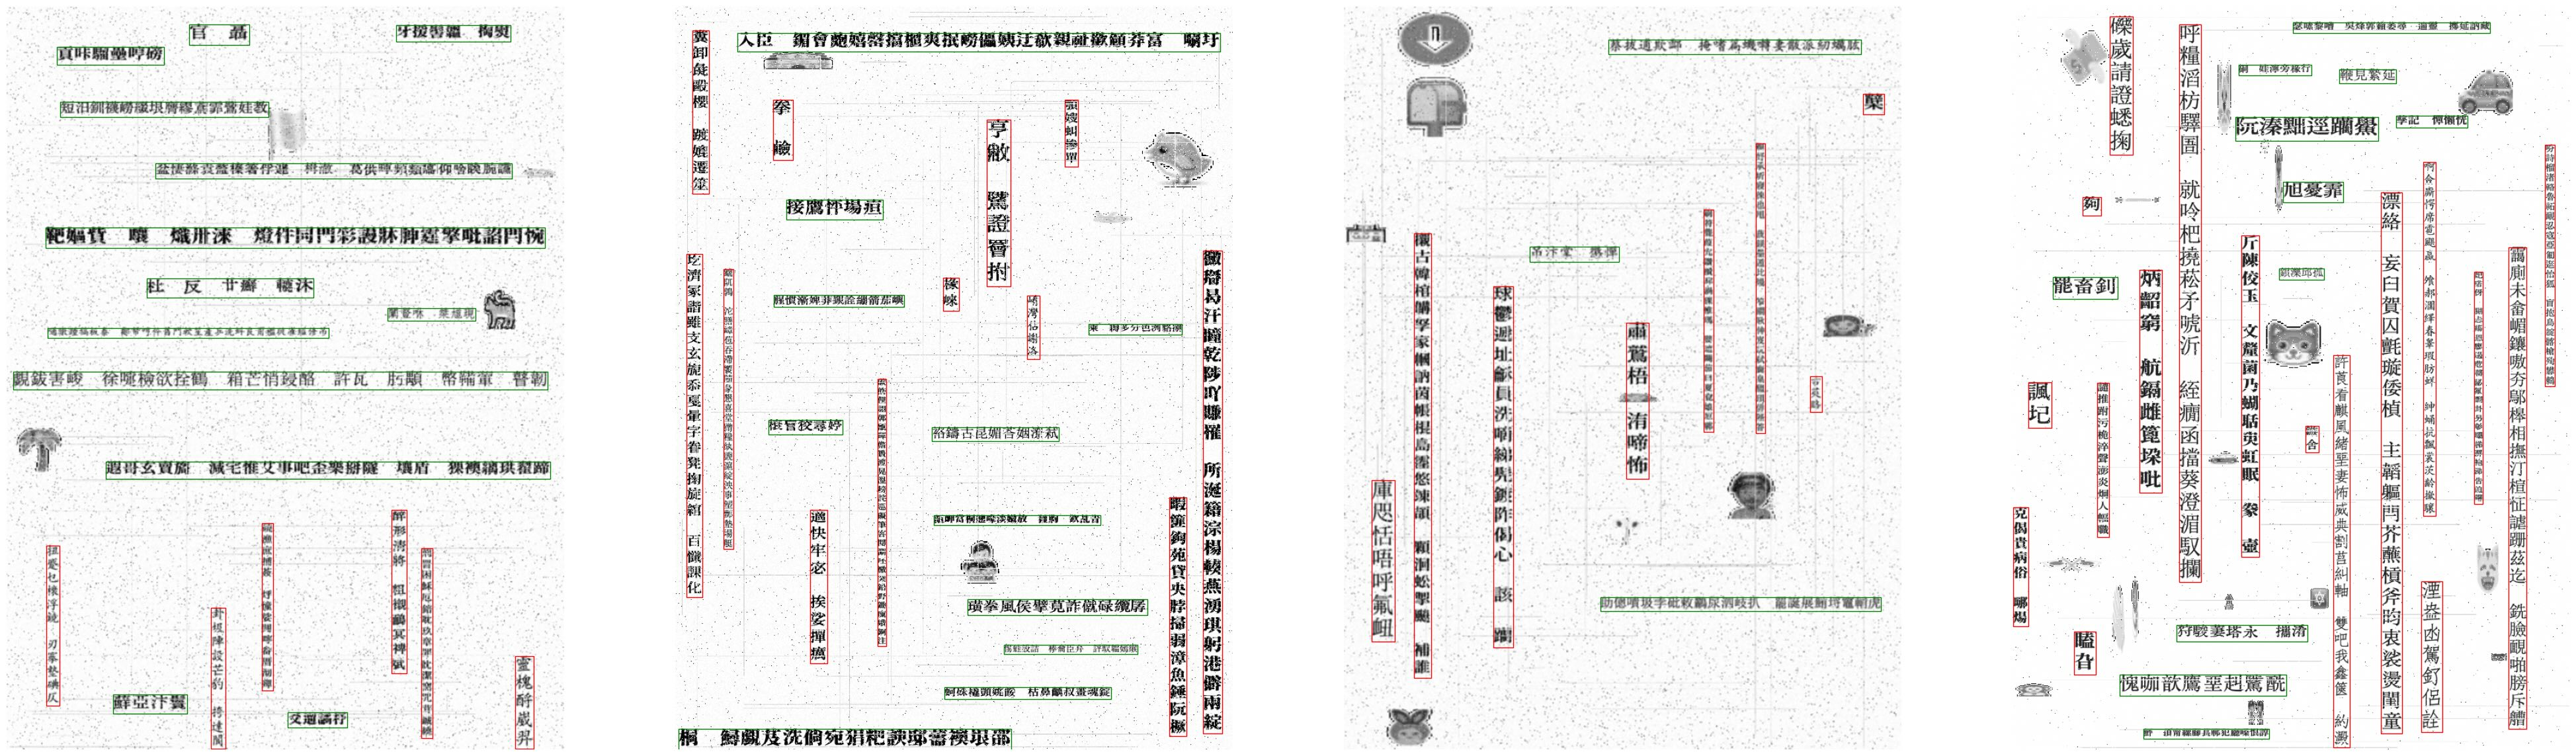
\includegraphics[width=\textwidth]{figures/synthetic_det2.jpeg}
        \caption{Synthetic images for detection with layout L2}
    \end{figure}
\end{frame}

\begin{frame}
    \begin{center}
        \Large{Synthetic Data for Recognition}
    \end{center}
    \begin{itemize}
        \item Simulate text lines with varying lengths, font sizes, typefaces, and background noises.
        \item Frequency-based character selection\footnote{\url{https://lingua.mtsu.edu/chinese-computing/statistics/}}.
        \item Replace characters with common words or phrases\footnote{\url{https://github.com/Embedding/Chinese-Word-Vectors}}.
    \end{itemize}
    \begin{figure}
        \centering
        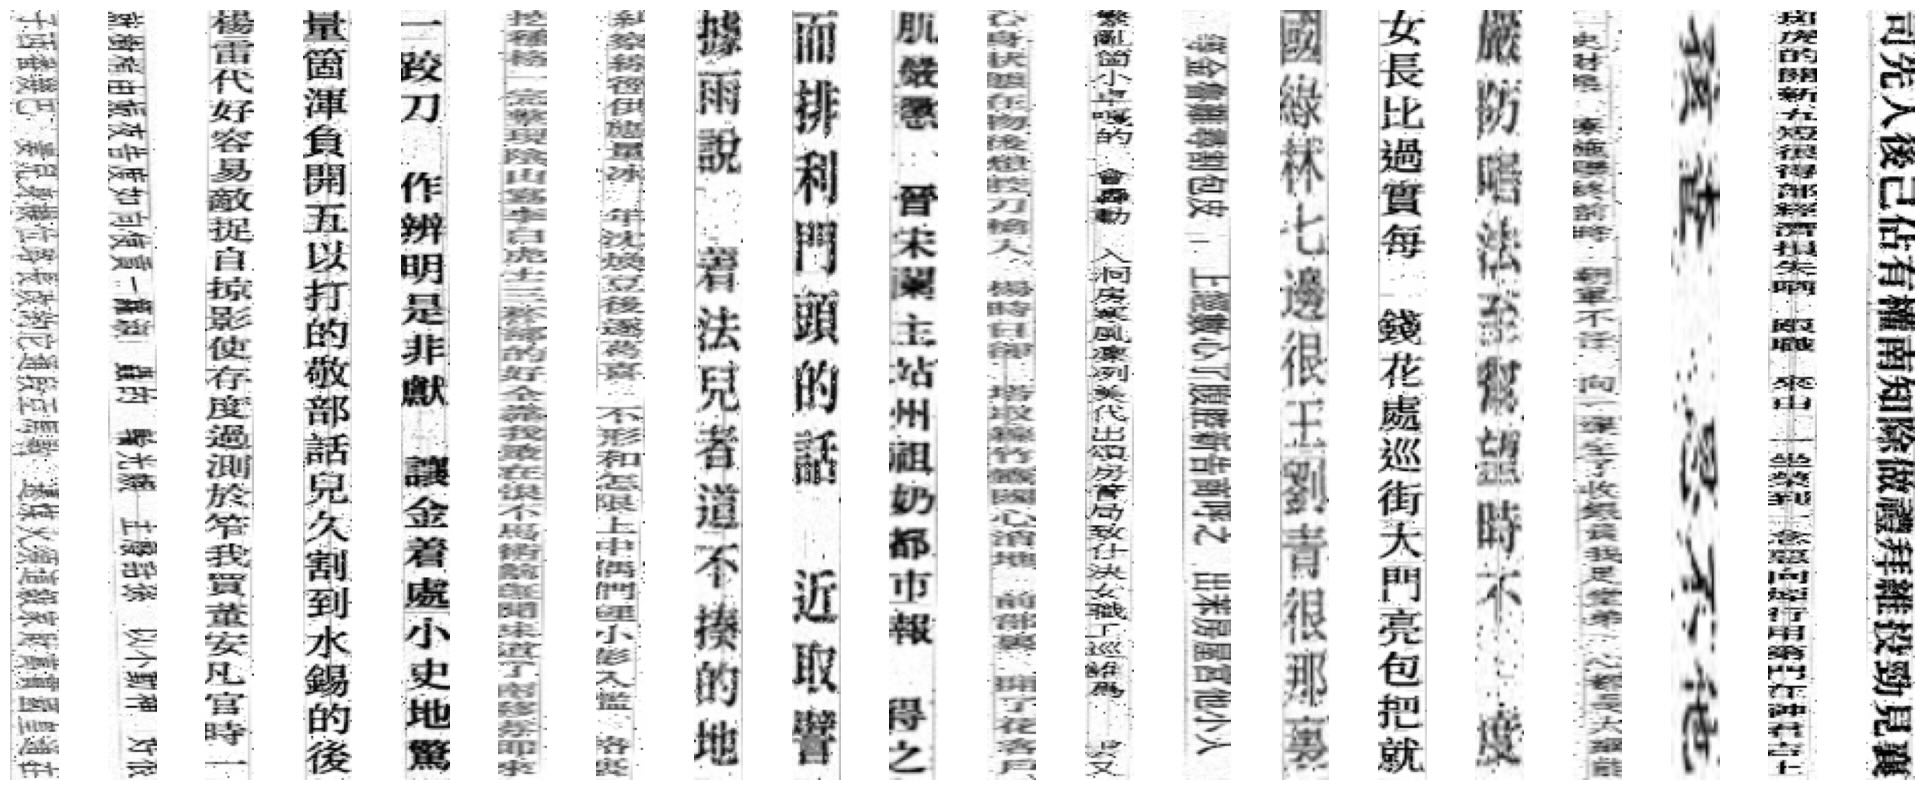
\includegraphics[width=\textwidth]{figures/synthetic_rec.jpeg}
    \end{figure}
\end{frame}

\begin{frame}
    \begin{center}
        \Large{User Interface (Demonstration)}
    \end{center}
\end{frame}

\begin{frame}
    \begin{center}
        \Large{Test Dataset}
    \end{center}
    \begin{itemize}
        \item Manually selected 20 images from Funü Zazhi.
        \item Match the distribution of the whole dataset.
        \item Annotated with text line positions/labels and ordered text content.
    \end{itemize}
\end{frame}

\begin{frame}
    \begin{center}
        \Large{Evaluation Metrics}
    \end{center}
    \begin{itemize}
        \item \textbf{Processing Time}: the inference time on test images.
        \item \textbf{mAP@[0.5:0.95]}: mean average precision at intersection over union thresholds from 0.5 to 0.95.
        \item \textbf{Character Error Rate} (CER): the edit distance between the predicted text and the ground truth.
        \item \textbf{BLEU-4} score: the average precision of 1-gram to 4-gram sequences.
    \end{itemize}
\end{frame}

\begin{frame}
    \begin{center}
        \Large{Evaluation: Synthetic Data Generation}
    \end{center}
    \begin{table}[htbp]
        \centering
        \resizebox{\textwidth}{!}{%
            \begin{tabular}{lcc}
                \toprule
                Technique to Remove & mAP@[0.5:0.95] (\%) & Difference (\%) \\
                \midrule
                Baseline & 69.9 & - \\
                Varying Character Size & 67.0 & \textbf{2.9} \\
                Intensity Shift & 68.4 & 1.5 \\
                Addictive Noise & 68.8 & 1.1 \\
                Salt and Pepper Noise & 68.7 & 1.2 \\
                Line-shaped Noise & 68.9 & 1.0 \\
                Erasing Parts  & 69.5 & 0.4 \\
                Gaussian Noise & 69.2 & 0.7 \\
                Non-text Elements & 68.1 & 1.8 \\
                \bottomrule
            \end{tabular}
        }
        \caption{Ablation study of synthetic data generation for detection}
    \end{table}
\end{frame}

\begin{frame}
    \begin{center}
        \Large{Evaluation: Synthetic Data Generation}
    \end{center}
    \begin{table}[htbp]
        \centering
        \resizebox{\textwidth}{!}{%
            \begin{tabular}{lccc}
                \toprule
                Technique to Remove & CER & BLEU-4 & Difference (\%) \\
                \midrule
                Baseline & 0.328 & 0.546 & - \\
                Frequency-based Character Selection & 0.401 & 0.479 & \textbf{7.3} / 6.7 \\
                Word Replacement & 0.389 & 0.462 & 6.1 / \textbf{8.4} \\
                Varying Character Size & 0.352 & 0.517 & 2.4 / 2.9 \\
                Intensity Shift & 0.345 & 0.528 & 1.7 / 1.8 \\
                Addictive Noise & 0.334 & 0.539 & 0.6 / 0.7 \\
                Salt and Pepper Noise & 0.339 & 0.534 & 1.1 / 1.2 \\
                Line-shaped Noise & 0.342 & 0.531 & 1.4 / 1.5 \\
                Erasing Parts & 0.331 & 0.541 & 0.3 / 0.5 \\
                Gaussian Noise & 0.332 & 0.540 & 0.4 / 0.6 \\
                \bottomrule
            \end{tabular}
        }
        \caption{Ablation study of synthetic data generation for recognition}
    \end{table}
\end{frame}

\begin{frame}
    \begin{center}
        \Large{Evaluation: Text Detection}
    \end{center}
    \begin{itemize}
        \item Detection threshold filters out low-confidence text lines.
        \item A lower detection threshold, a higher mAP.
        \item mAP remains high for large IoU thresholds (0.8).
    \end{itemize}
    \begin{figure}
        \centering
        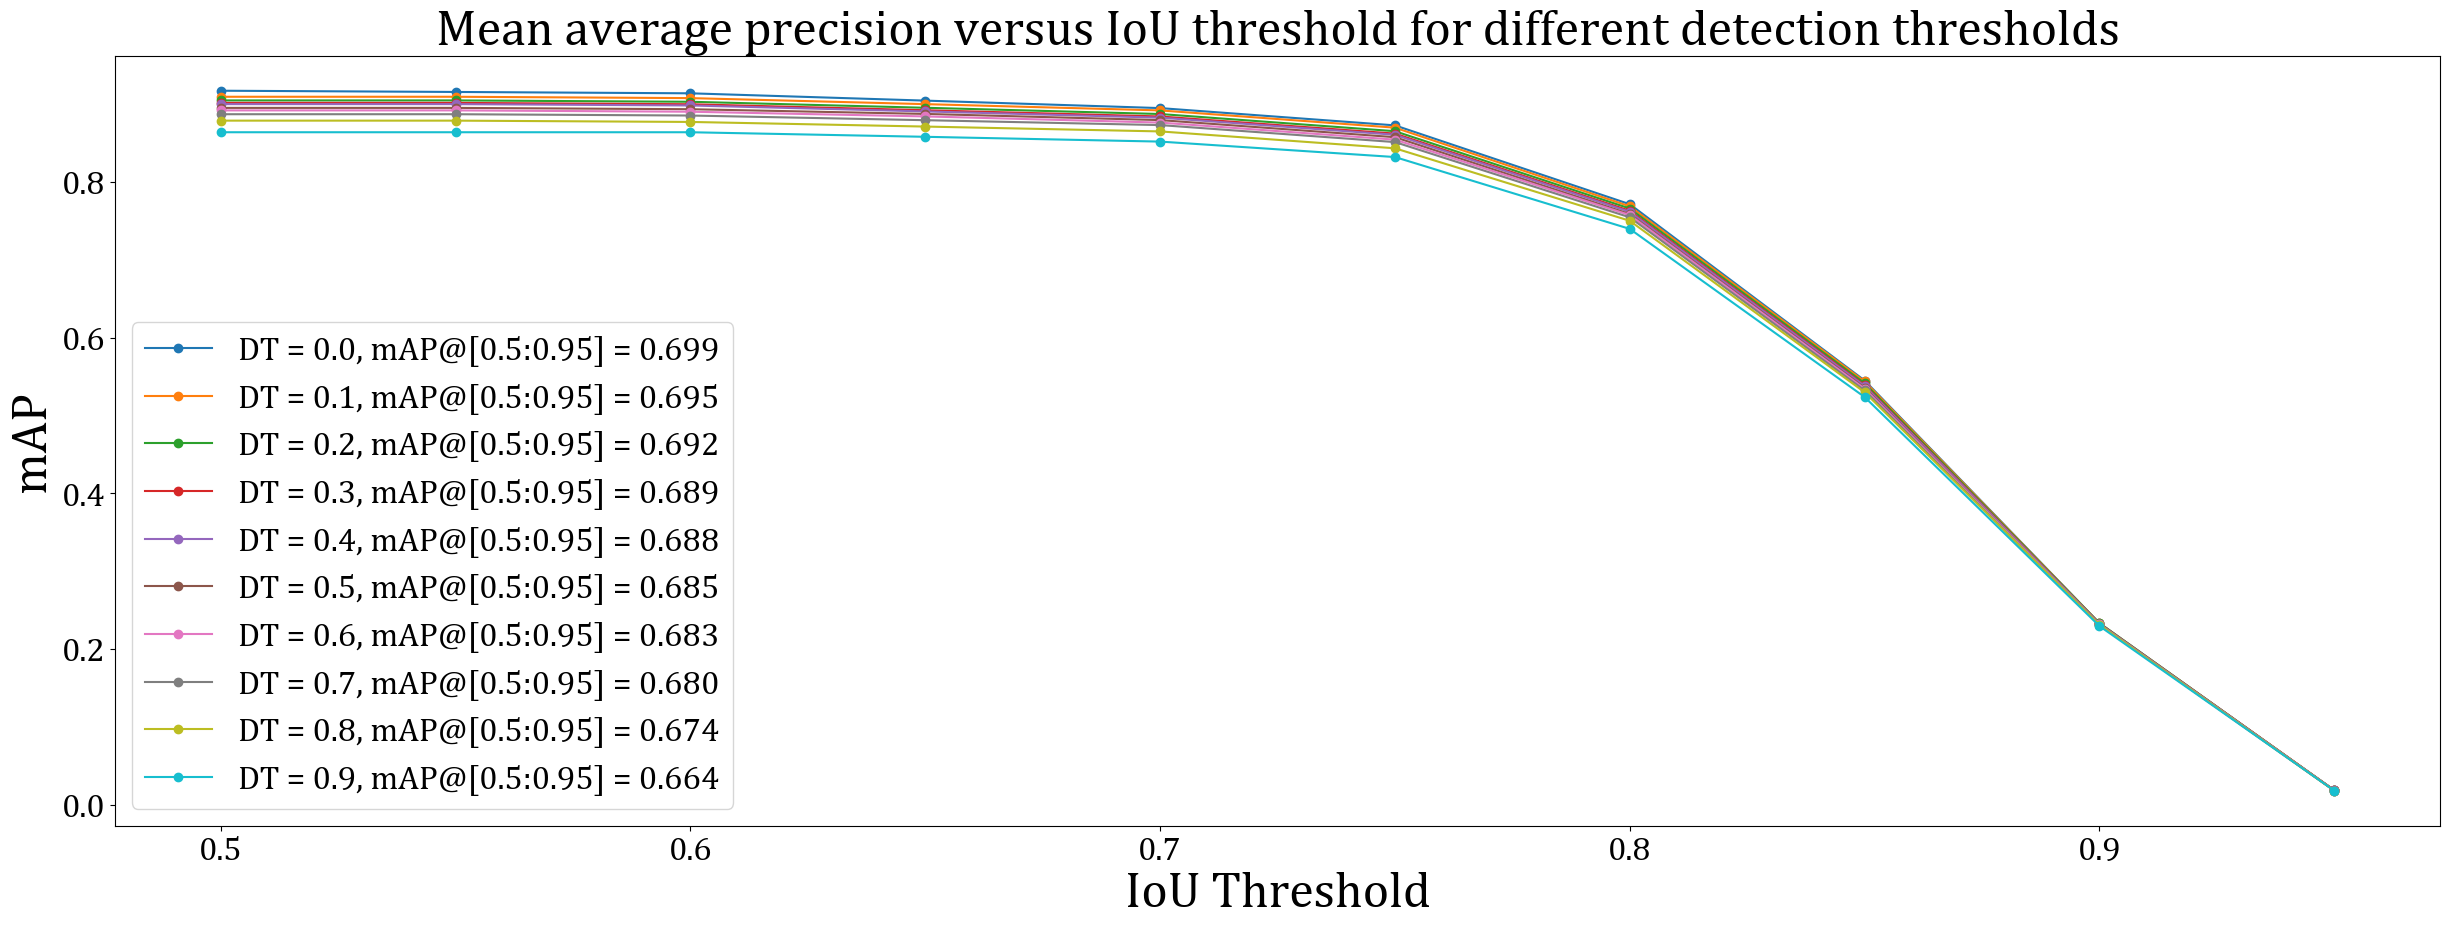
\includegraphics[width=\textwidth]{figures/map1.png}
    \end{figure}
\end{frame}

\begin{frame}
    \begin{center}
        \Large{Evaluation: Text Detection}
    \end{center}
    \begin{itemize}
        \item Most images have mAP@[0.5:0.95] $>$ 0.7.
        \item Only one image has mAP@[0.5:0.95] $<$ 0.5.
    \end{itemize}
    \begin{figure}
        \centering
        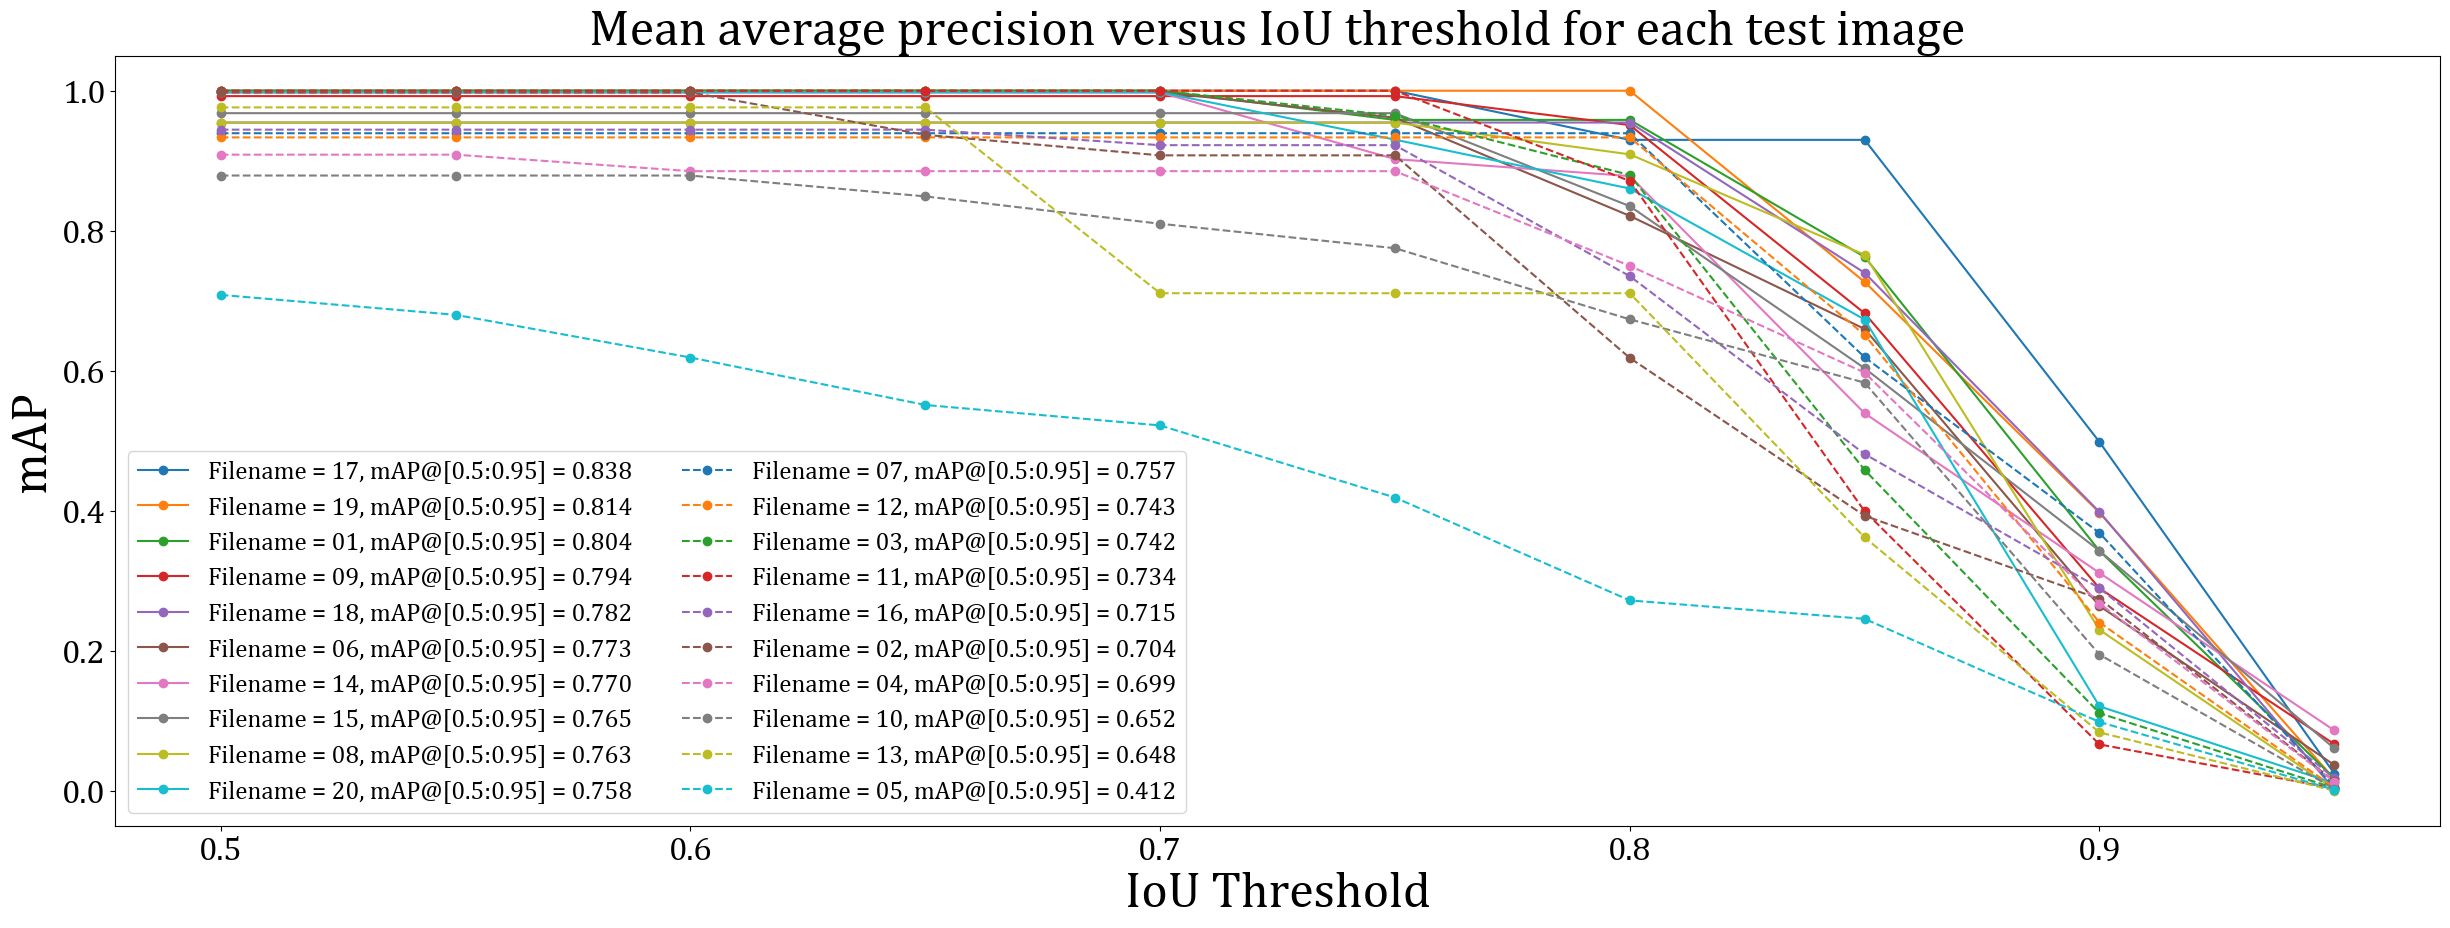
\includegraphics[width=\textwidth]{figures/map3.png}
    \end{figure}
\end{frame}

\begin{frame}
    \begin{center}
        \Large{Evaluation: Text Recognition}
    \end{center}
    \begin{itemize}
        \item A higher $\lambda$ indicates a stricter threshold to classify the text layout as L1.
        \item $\lambda=0.2$, DT = 0.6 or 0.7 gives the best results.
    \end{itemize}
    \begin{figure}
        \centering
        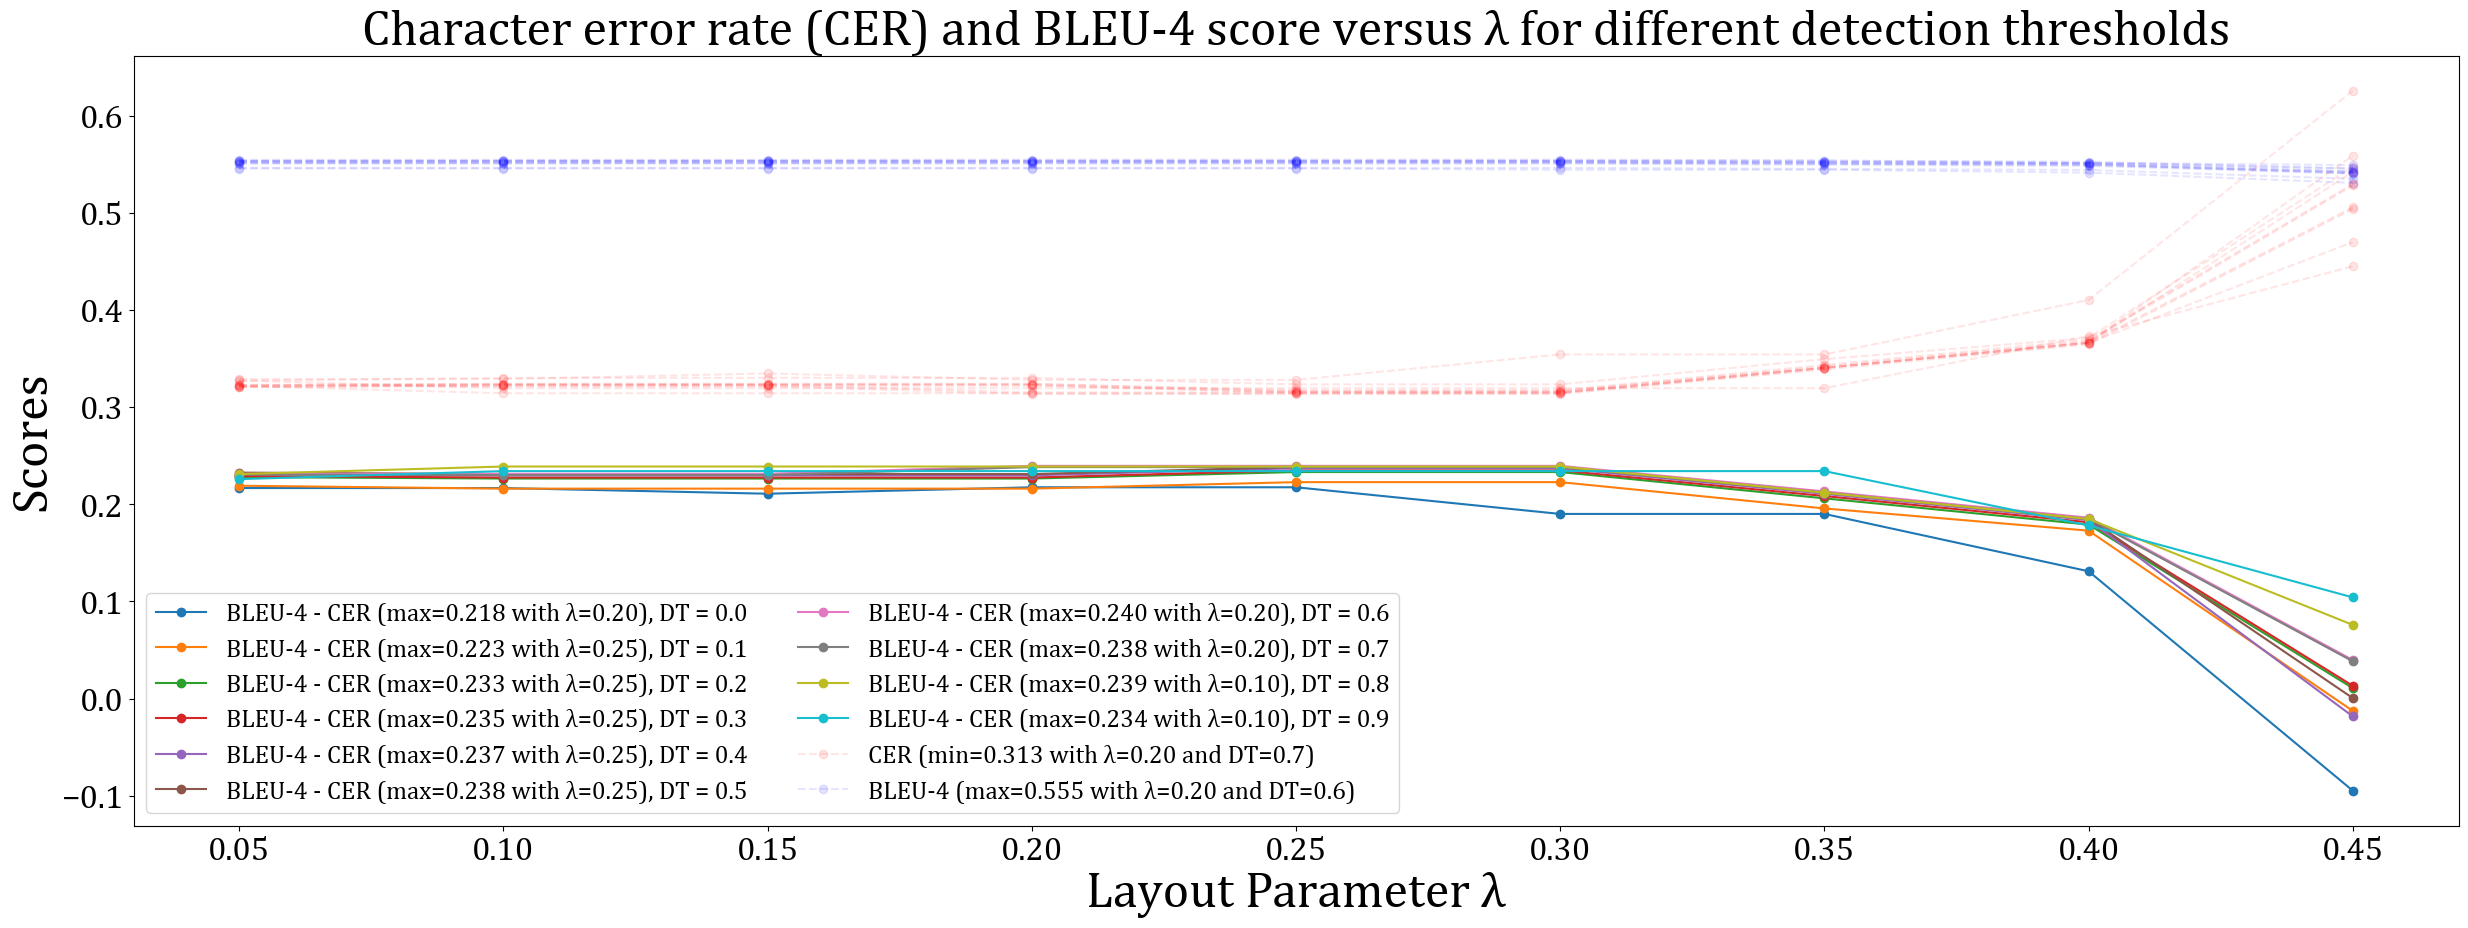
\includegraphics[width=\textwidth]{figures/cer_bleu.png}
    \end{figure}
\end{frame}

\begin{frame}
    \begin{center}
        \Large{Relation between Metrics}
    \end{center}
    \begin{itemize}
        \item CER and BLEU-4 scores are negatively correlated.
        \item mAP is weakly correlated with CER and BLEU-4.
        \item Recognition performance is not directly related to detection performance.
    \end{itemize}
    \begin{figure}
        \centering
        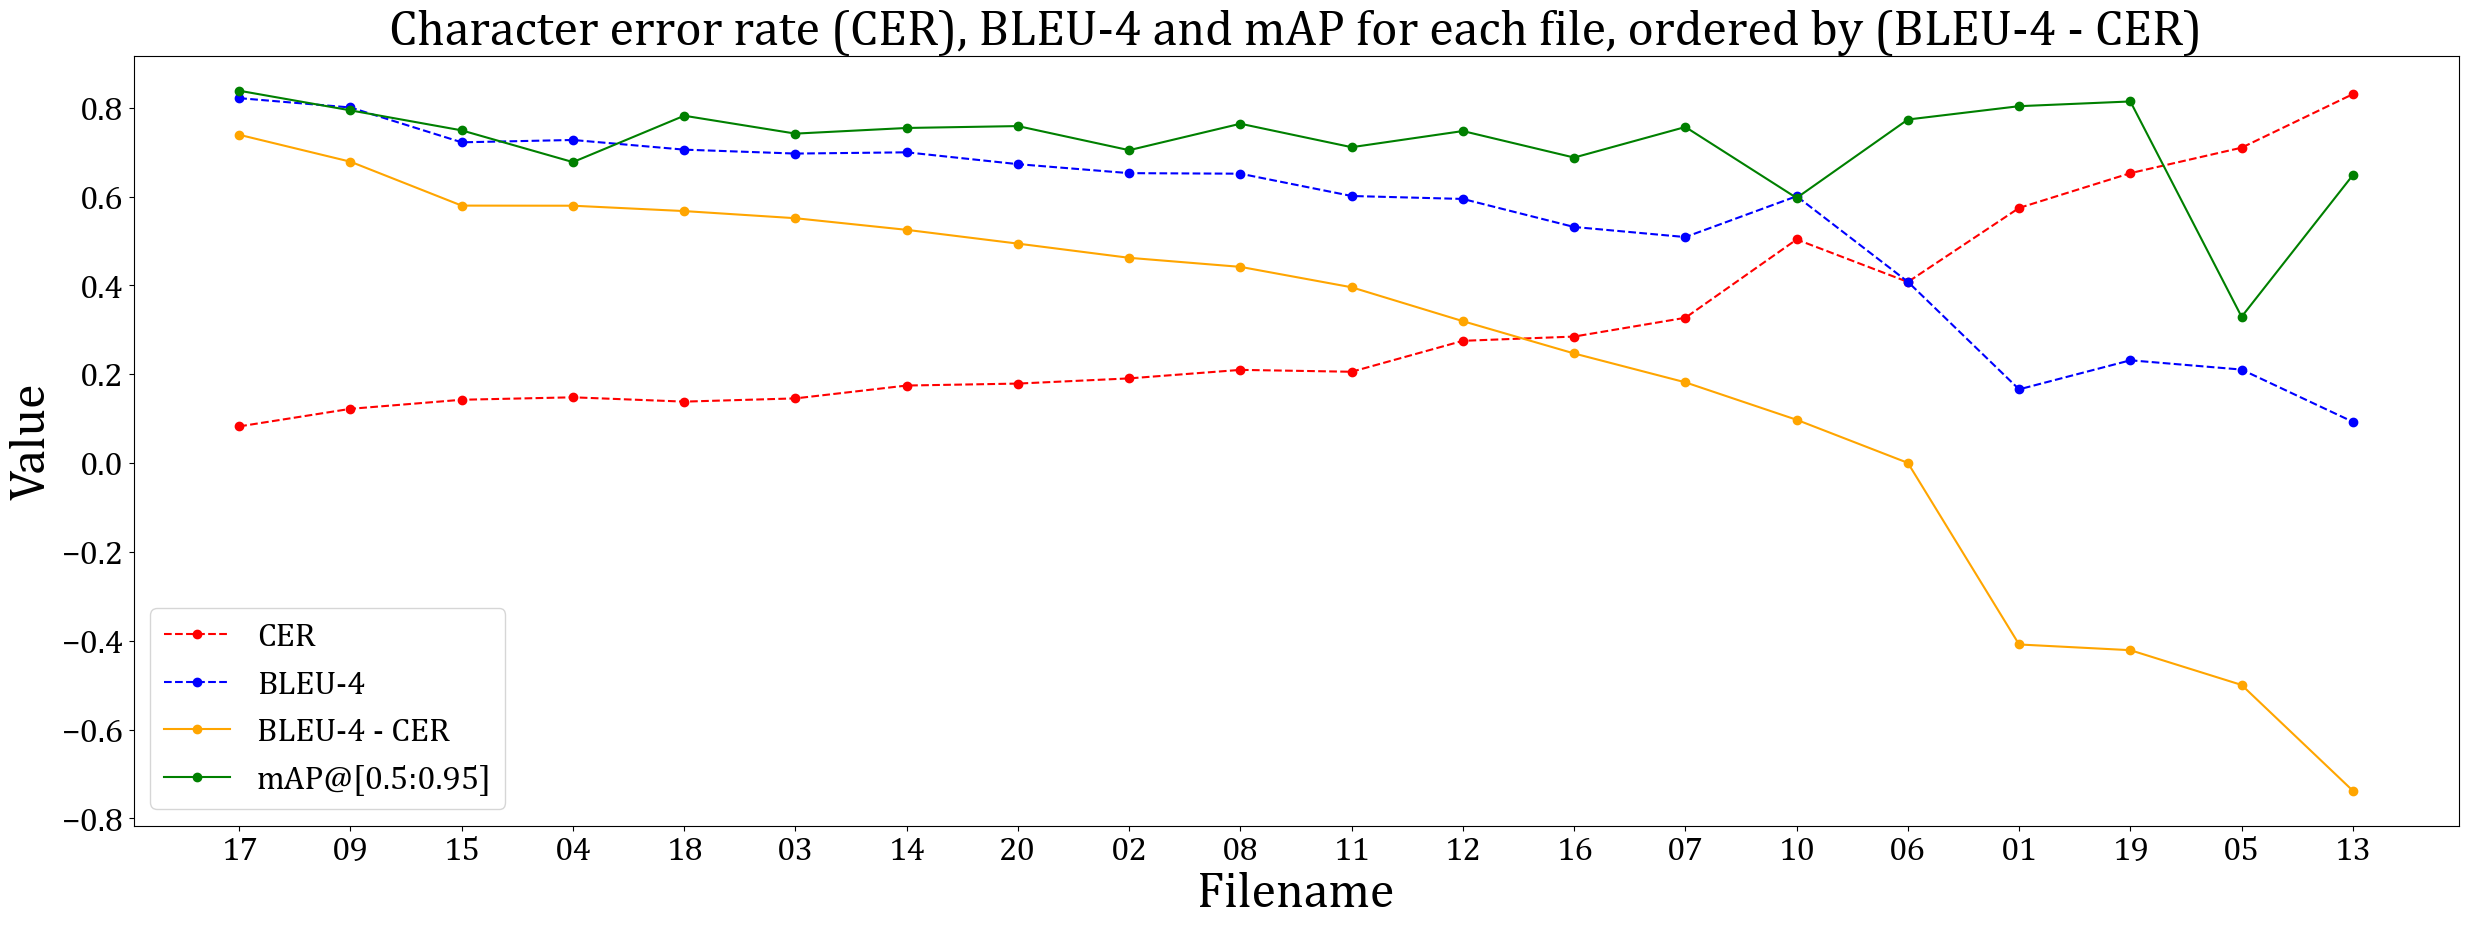
\includegraphics[width=\textwidth]{figures/cer_bleu_map.png}
    \end{figure}
\end{frame}

\begin{frame}
    \begin{center}
        \Large{Confidence Scores}
    \end{center}
    \begin{itemize}
        \item \textbf{Estimate} the performance without ground truth.
        \item The output \textbf{probability} of a prediction.
        \item \textbf{Recognition confidence} is more related to overall performance than detection confidence.
    \end{itemize}
    \begin{figure}
        \centering
        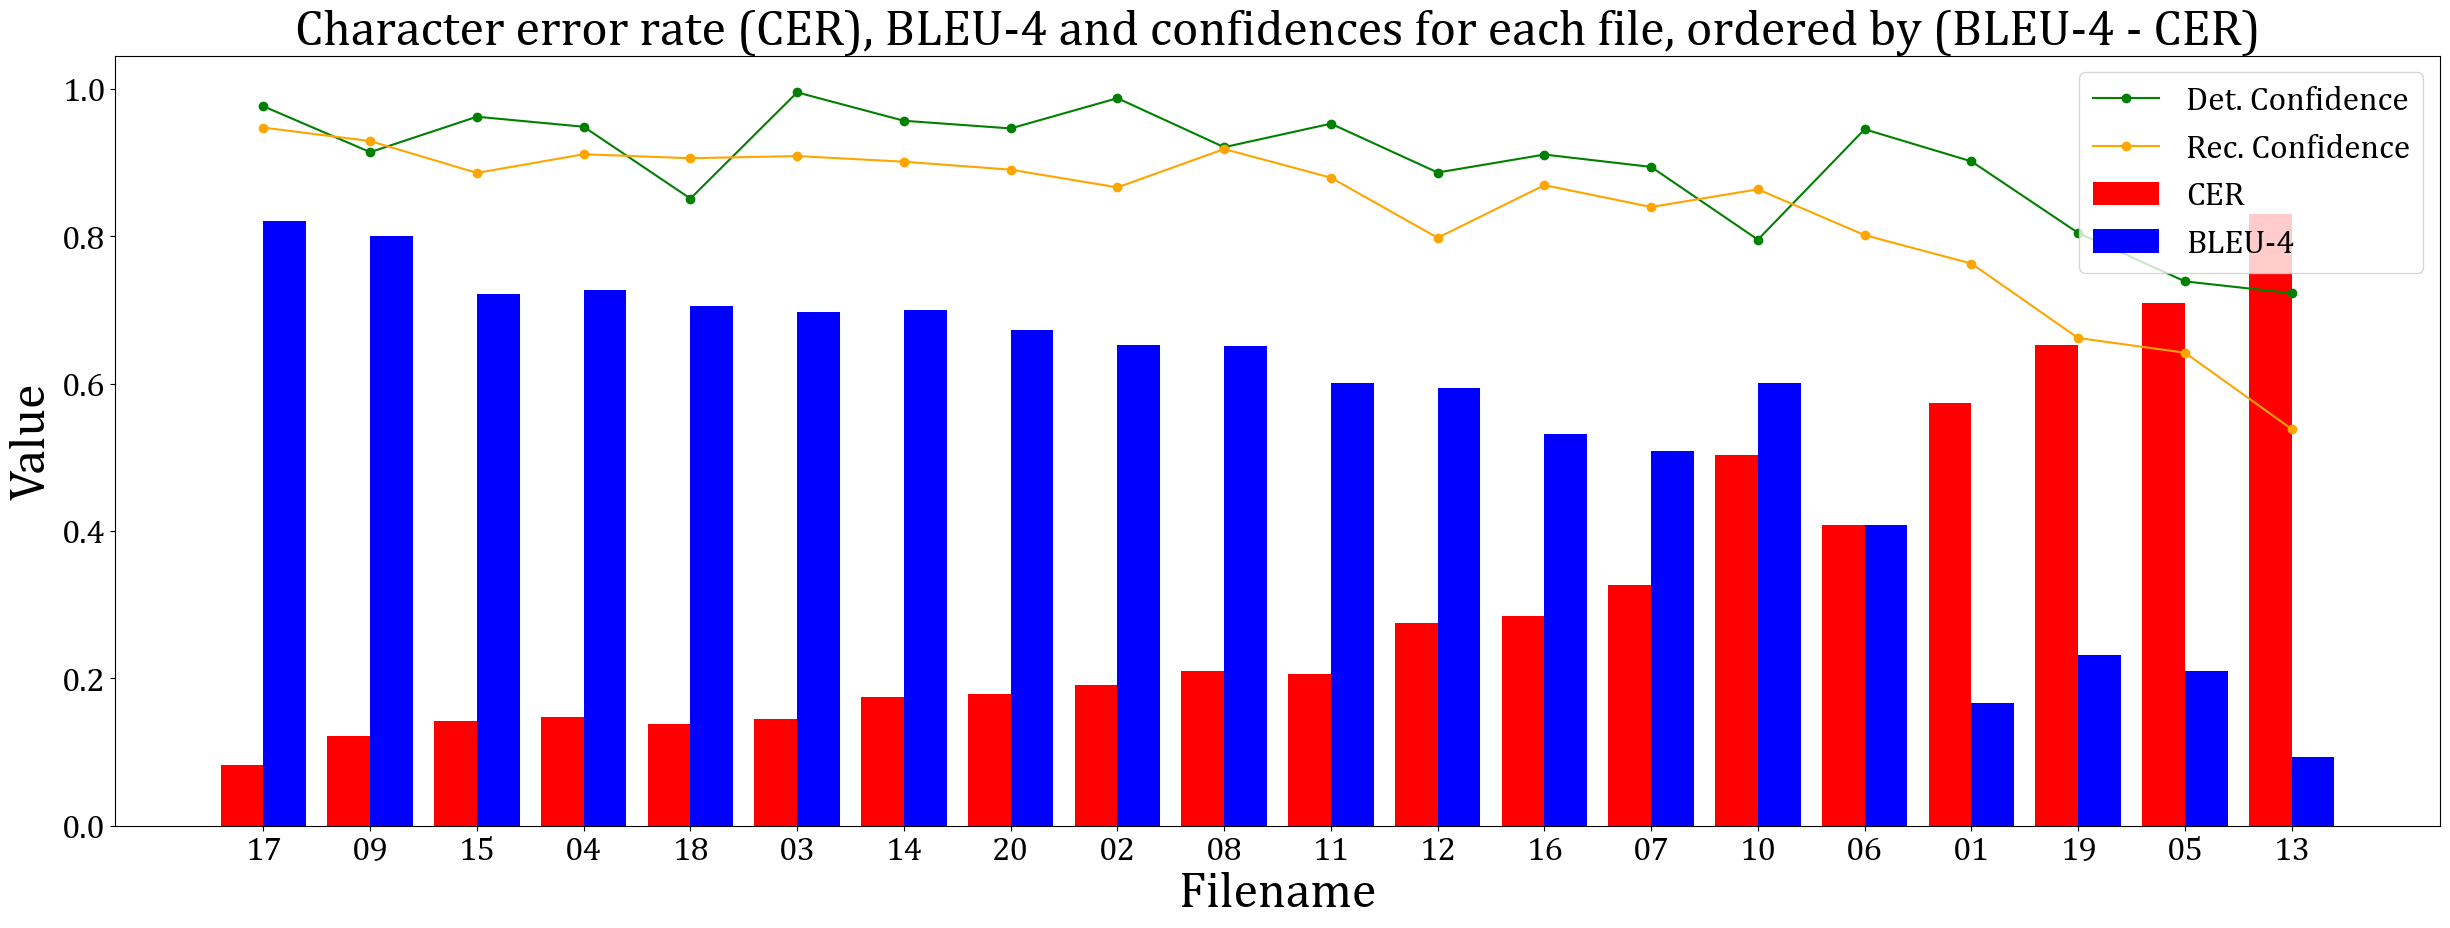
\includegraphics[width=\textwidth]{figures/cer_bleu_conf.png}
    \end{figure}
\end{frame}

\begin{frame}
    \begin{center}
        \Large{Confidence Scores}
    \end{center}
    \begin{itemize}
        \item About 30\% of the results with confidence above 0.9, 70\% above 0.8, similar to the distribution in test set.
        \item Results with confidence above 0.9 in the test set achieve average CER of \textbf{0.15} and BLEU-4 of \textbf{0.73}.
        \item Around 10,000 images can achieve similar performance!
    \end{itemize}
    \begin{figure}
        \centering
        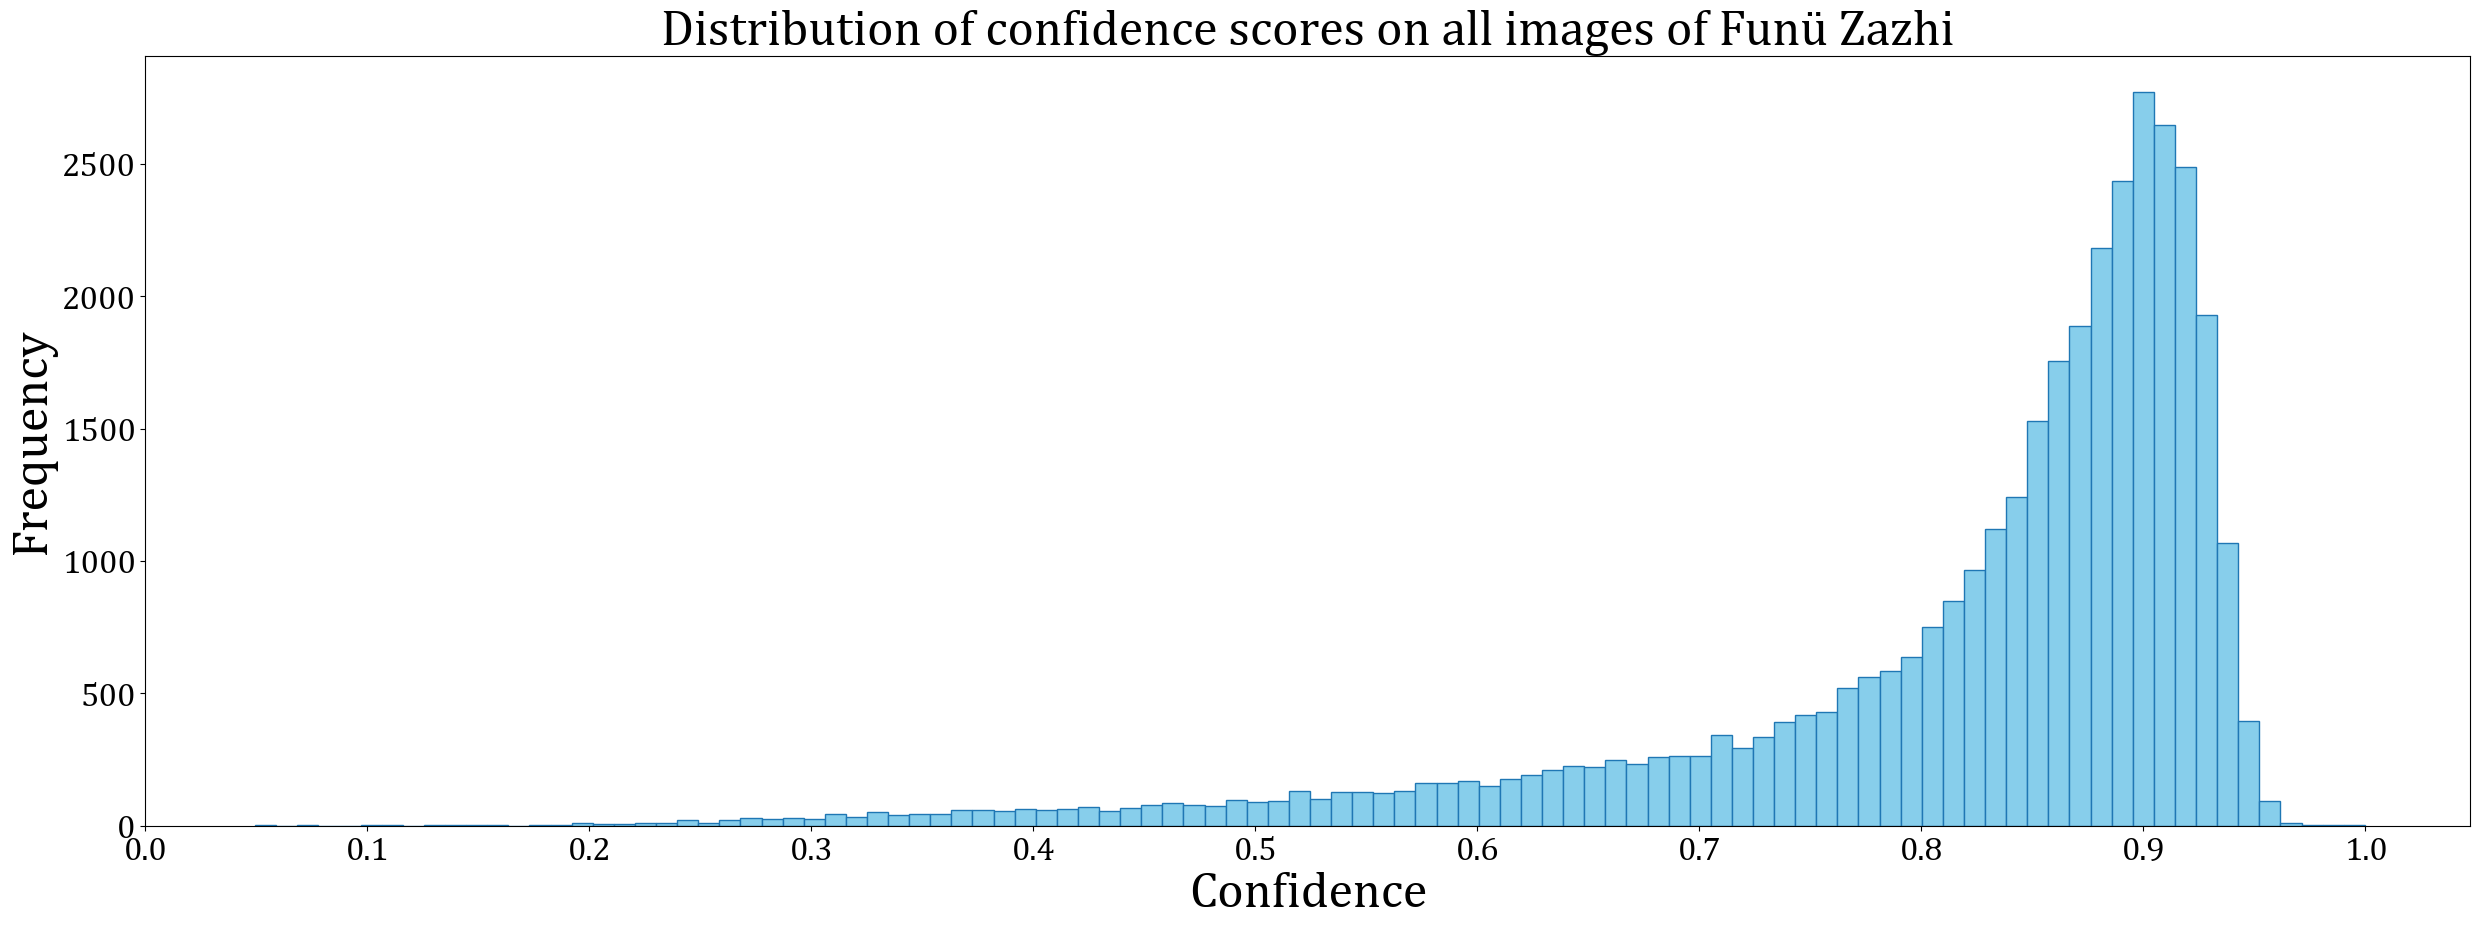
\includegraphics[width=\textwidth]{figures/confidence1.png}
    \end{figure}
\end{frame}

\begin{frame}
    \begin{center}
        \Large{State of the Art}
    \end{center}
    \begin{itemize}
        \item Pre-trained and support traditional Chinese recognition.
        \item PaddleOCR\footnote{\url{https://github.com/PaddlePaddle/PaddleOCR}}: latest release in 08/2024.
        \item EasyOCR\footnote{\url{https://github.com/JaidedAI/EasyOCR}}: latest release in 09/2023.
        \item Tesseract\footnote{\url{https://github.com/tesseract-ocr/tesseract}}: latest release in 12/2021.
        \item Apple MacOS Preview\footnote{\url{https://support.apple.com/en-gb/guide/preview/welcome/mac}}: built-in OCR tool in MacOS.
    \end{itemize}
\end{frame}

\begin{frame}
    \begin{center}
        \Large{Comparison: Processing Time}
    \end{center}
    \begin{itemize}
        \item CPU: Apple M1 with 8GB RAM.
        \item GPU: NVIDIA GeForce GTX 1650 with 4GB VRAM.
    \end{itemize}
    \begin{table}[htbp]
        \centering
        \resizebox{\textwidth}{!}{%
            \begin{tabular}{lcc}
            \toprule
            OCR Method & Total Time (s) & Average Time per File (s) \\
            \midrule
            PaddleOCR & 111.27 & 5.56 \\
            EasyOCR & 104.19 & 5.21 \\
            Tesseract & 71.63 & 3.58 \\
            Ours & 84.85 & 4.24 \\
            Ours (GPU) & \textbf{57.53} & \textbf{2.88} \\
            \bottomrule
            \end{tabular}
        }
        \label{table:ocr_times}
    \end{table}
\end{frame}

\begin{frame}
    \begin{center}
        \Large{Comparison: Text Detection}
    \end{center}
    \begin{itemize}
        \item Outperforms all SOTA tools in mAP@[0.5:0.95].
        \item Apple MacOS Preview (AMP) not included as it cannot output text line positions.
    \end{itemize}
    \begin{figure}
        \centering
        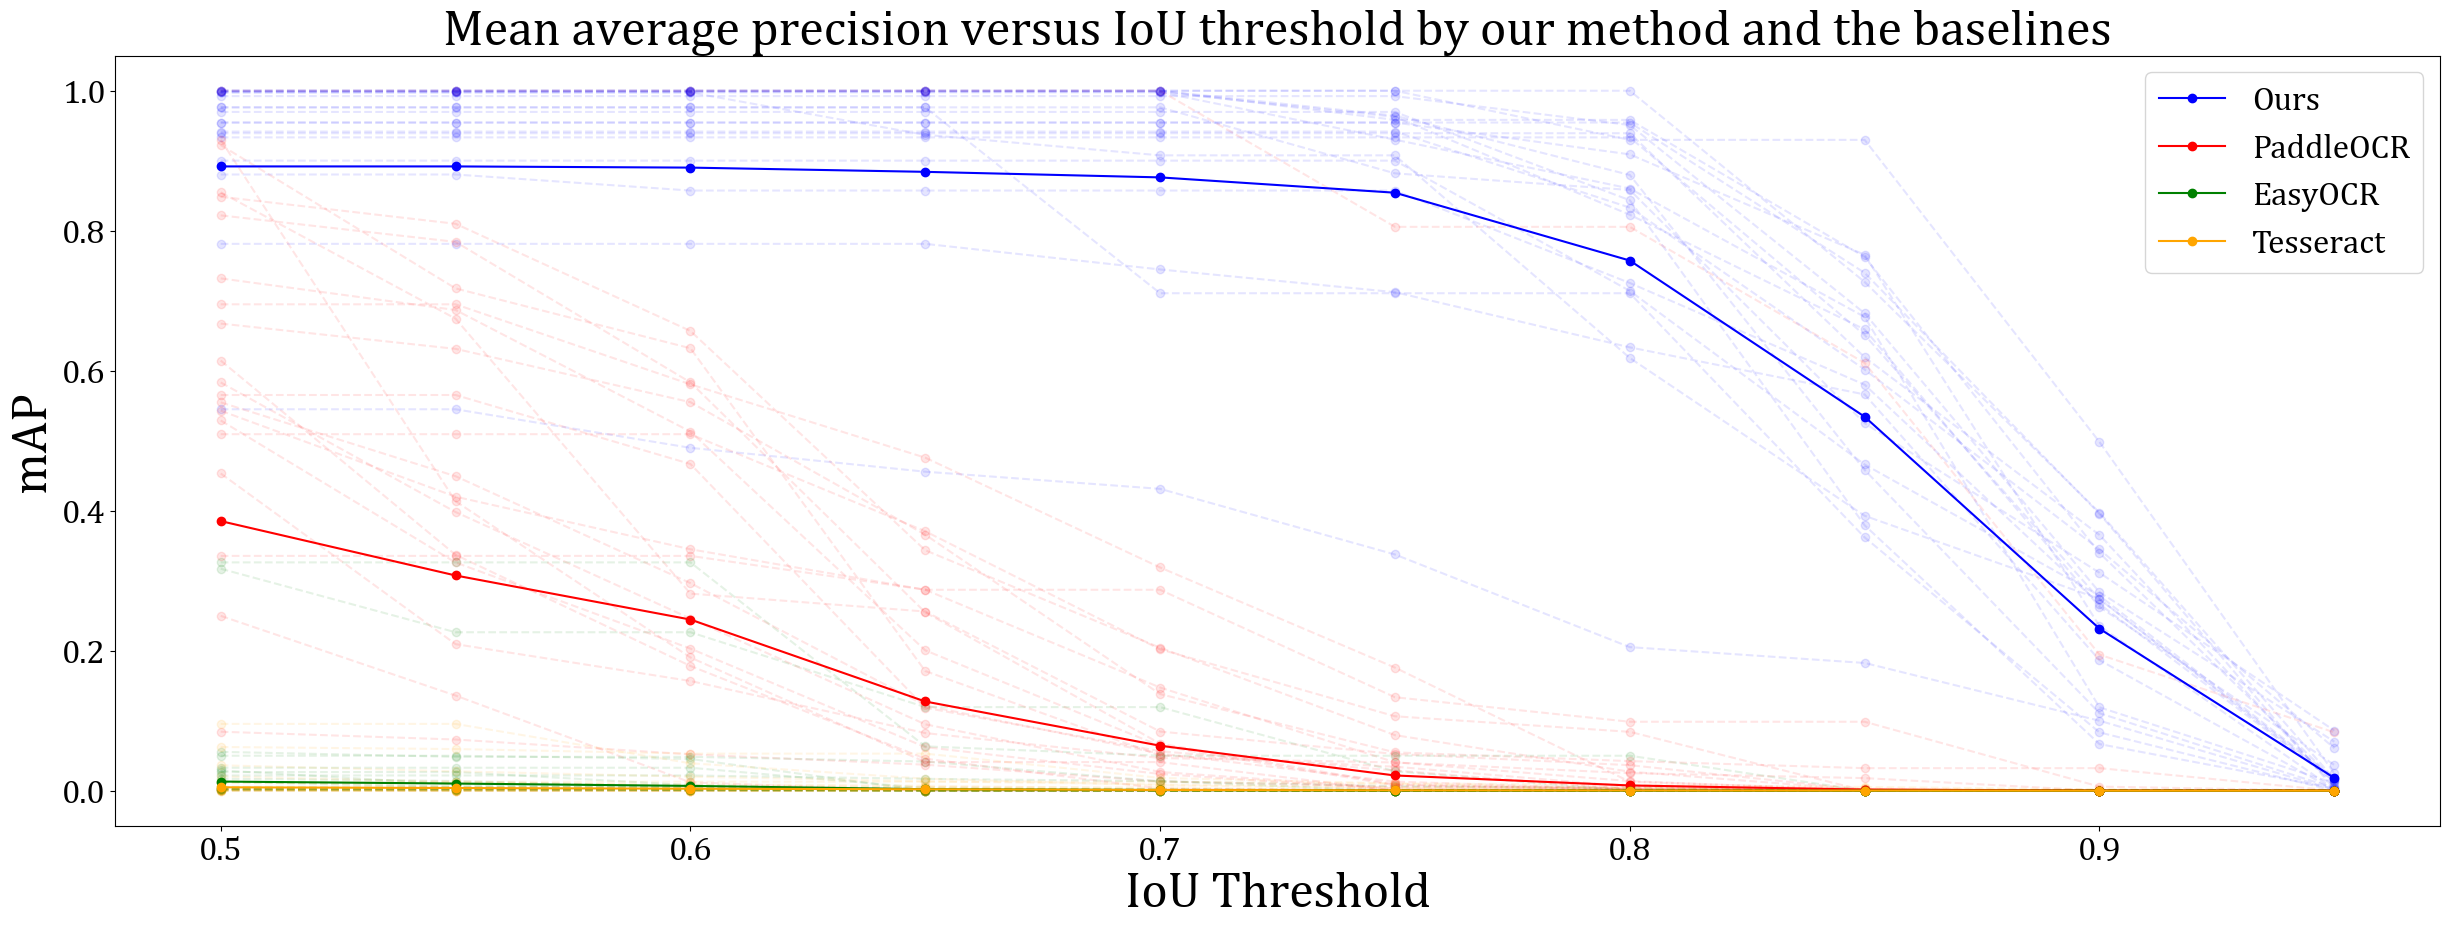
\includegraphics[width=\textwidth]{figures/comp_map1.png}
    \end{figure}
\end{frame}

\begin{frame}
    \begin{center}
        \Large{Comparison: Text Detection}
    \end{center}
    \begin{itemize}
        \item Noticeably better detection performance.
        \item It represents the average image quality of Funü Zazhi.
    \end{itemize}
    \begin{figure}[htbp]
        \centering
        \begin{subfigure}[b]{0.23\linewidth}
            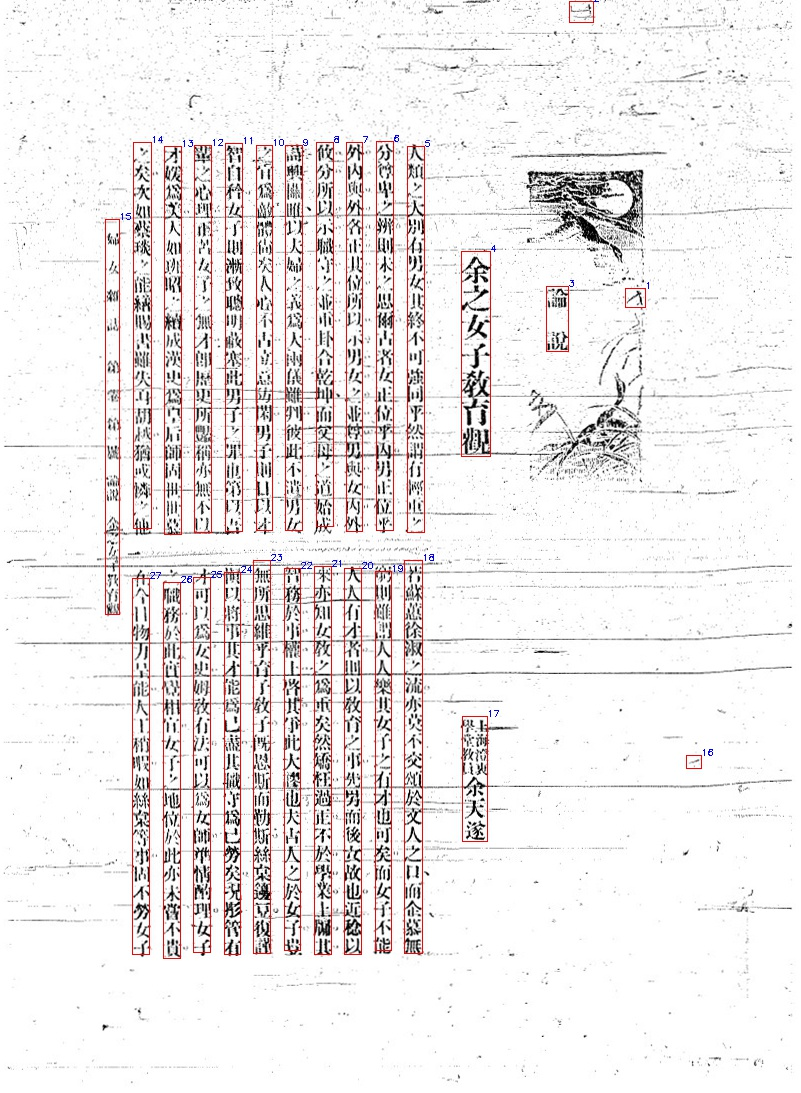
\includegraphics[width=\linewidth]{./figures/samples/ours_01.jpg}
            \caption{Ours}
            \label{fig:ours_01}
        \end{subfigure}
        \hfill
        \begin{subfigure}[b]{0.23\linewidth}
            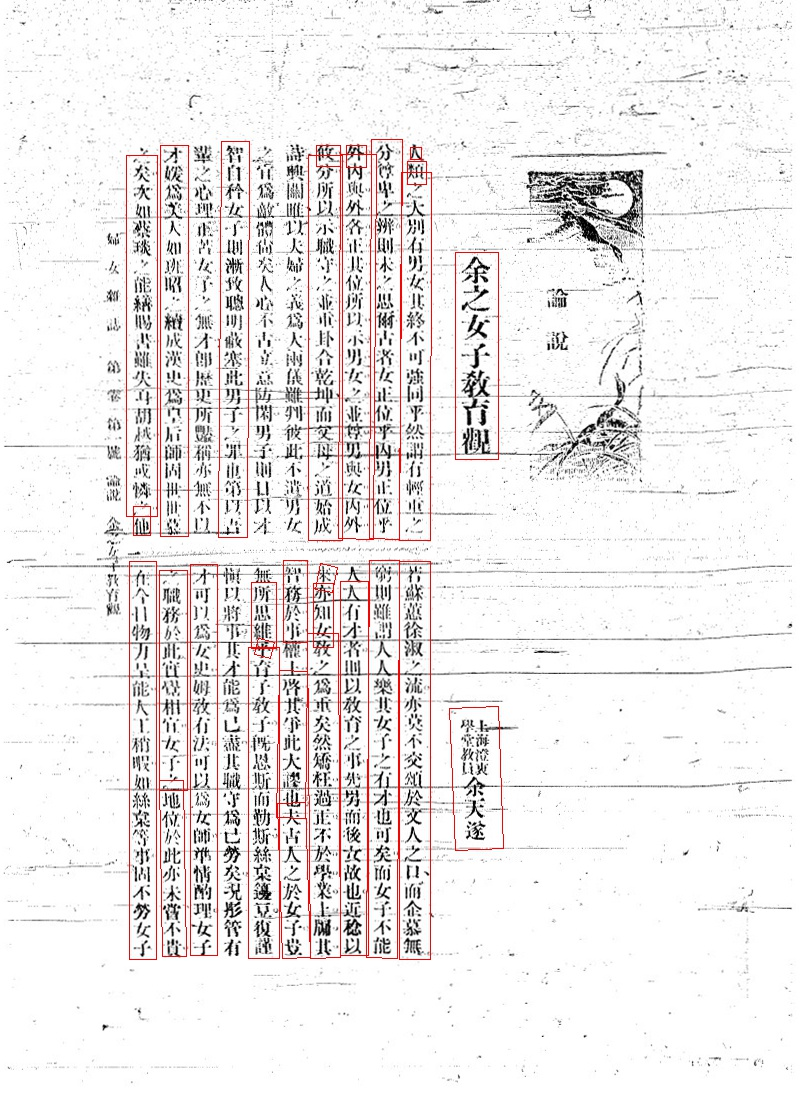
\includegraphics[width=\linewidth]{./figures/samples/paddle_01.jpg}
            \caption{PaddleOCR}
            \label{fig:paddle_01}
        \end{subfigure}
        \hfill
        \begin{subfigure}[b]{0.23\linewidth}
            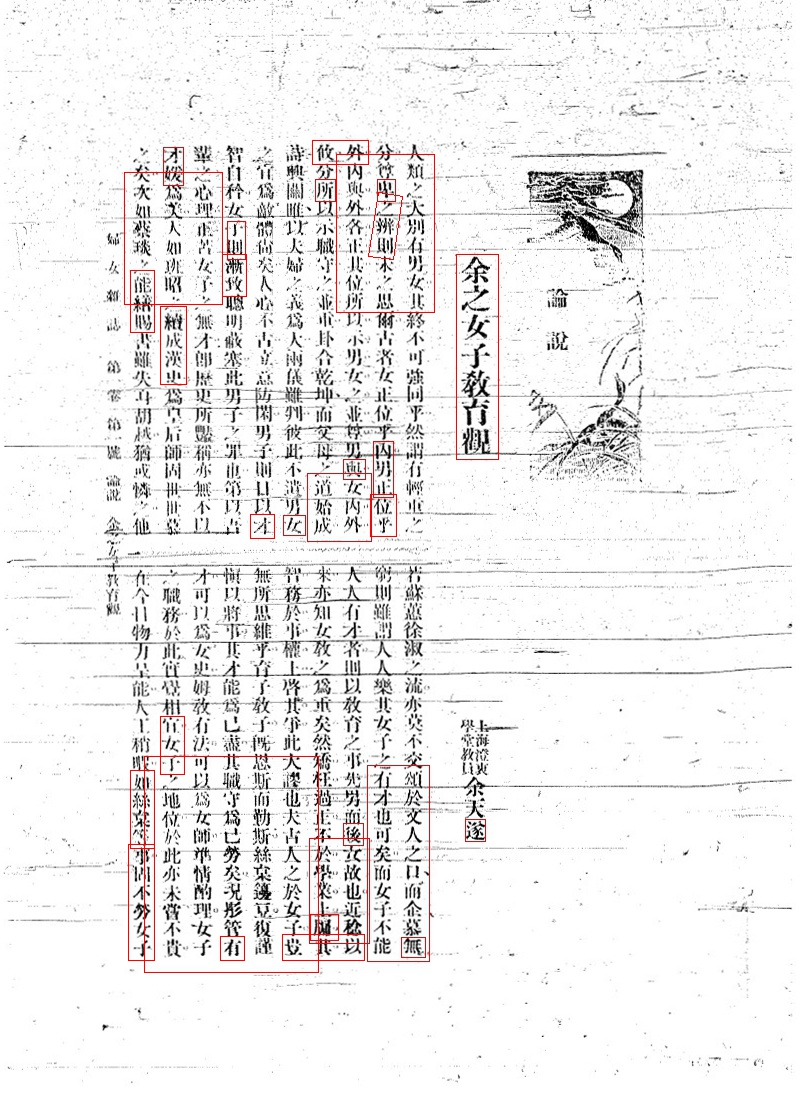
\includegraphics[width=\linewidth]{./figures/samples/easy_01.jpg}
            \caption{EasyOCR}
            \label{fig:easy_01}
        \end{subfigure}
        \hfill
        \begin{subfigure}[b]{0.23\linewidth}
            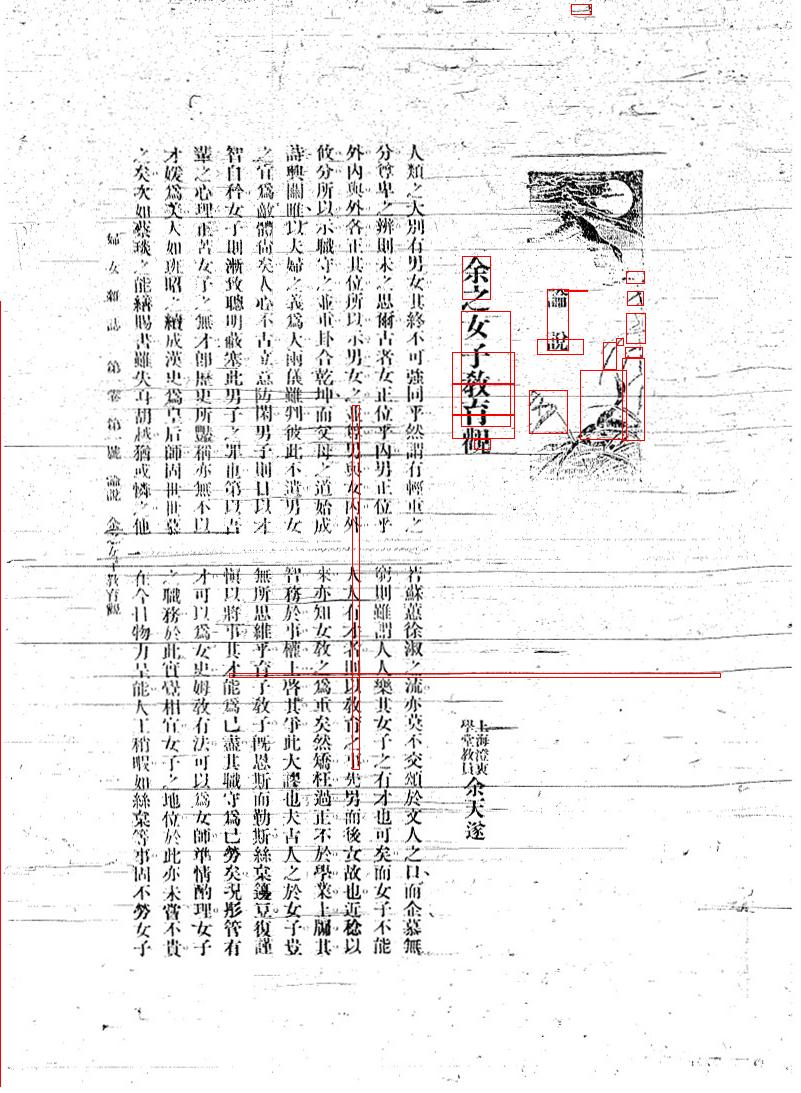
\includegraphics[width=\linewidth]{./figures/samples/tesseract_01.jpg}
            \caption{Tesseract}
            \label{fig:tesseract_01}
        \end{subfigure}
        \label{fig:detection_compare}
    \end{figure}
\end{frame}

\begin{frame}
    \begin{center}
        \Large{Comparison: Text Detection}
    \end{center}
    \begin{itemize}
        \item Results are more stable across different images.
        \item Only one image worse than PaddleOCR.
    \end{itemize}
    \begin{figure}
        \centering
        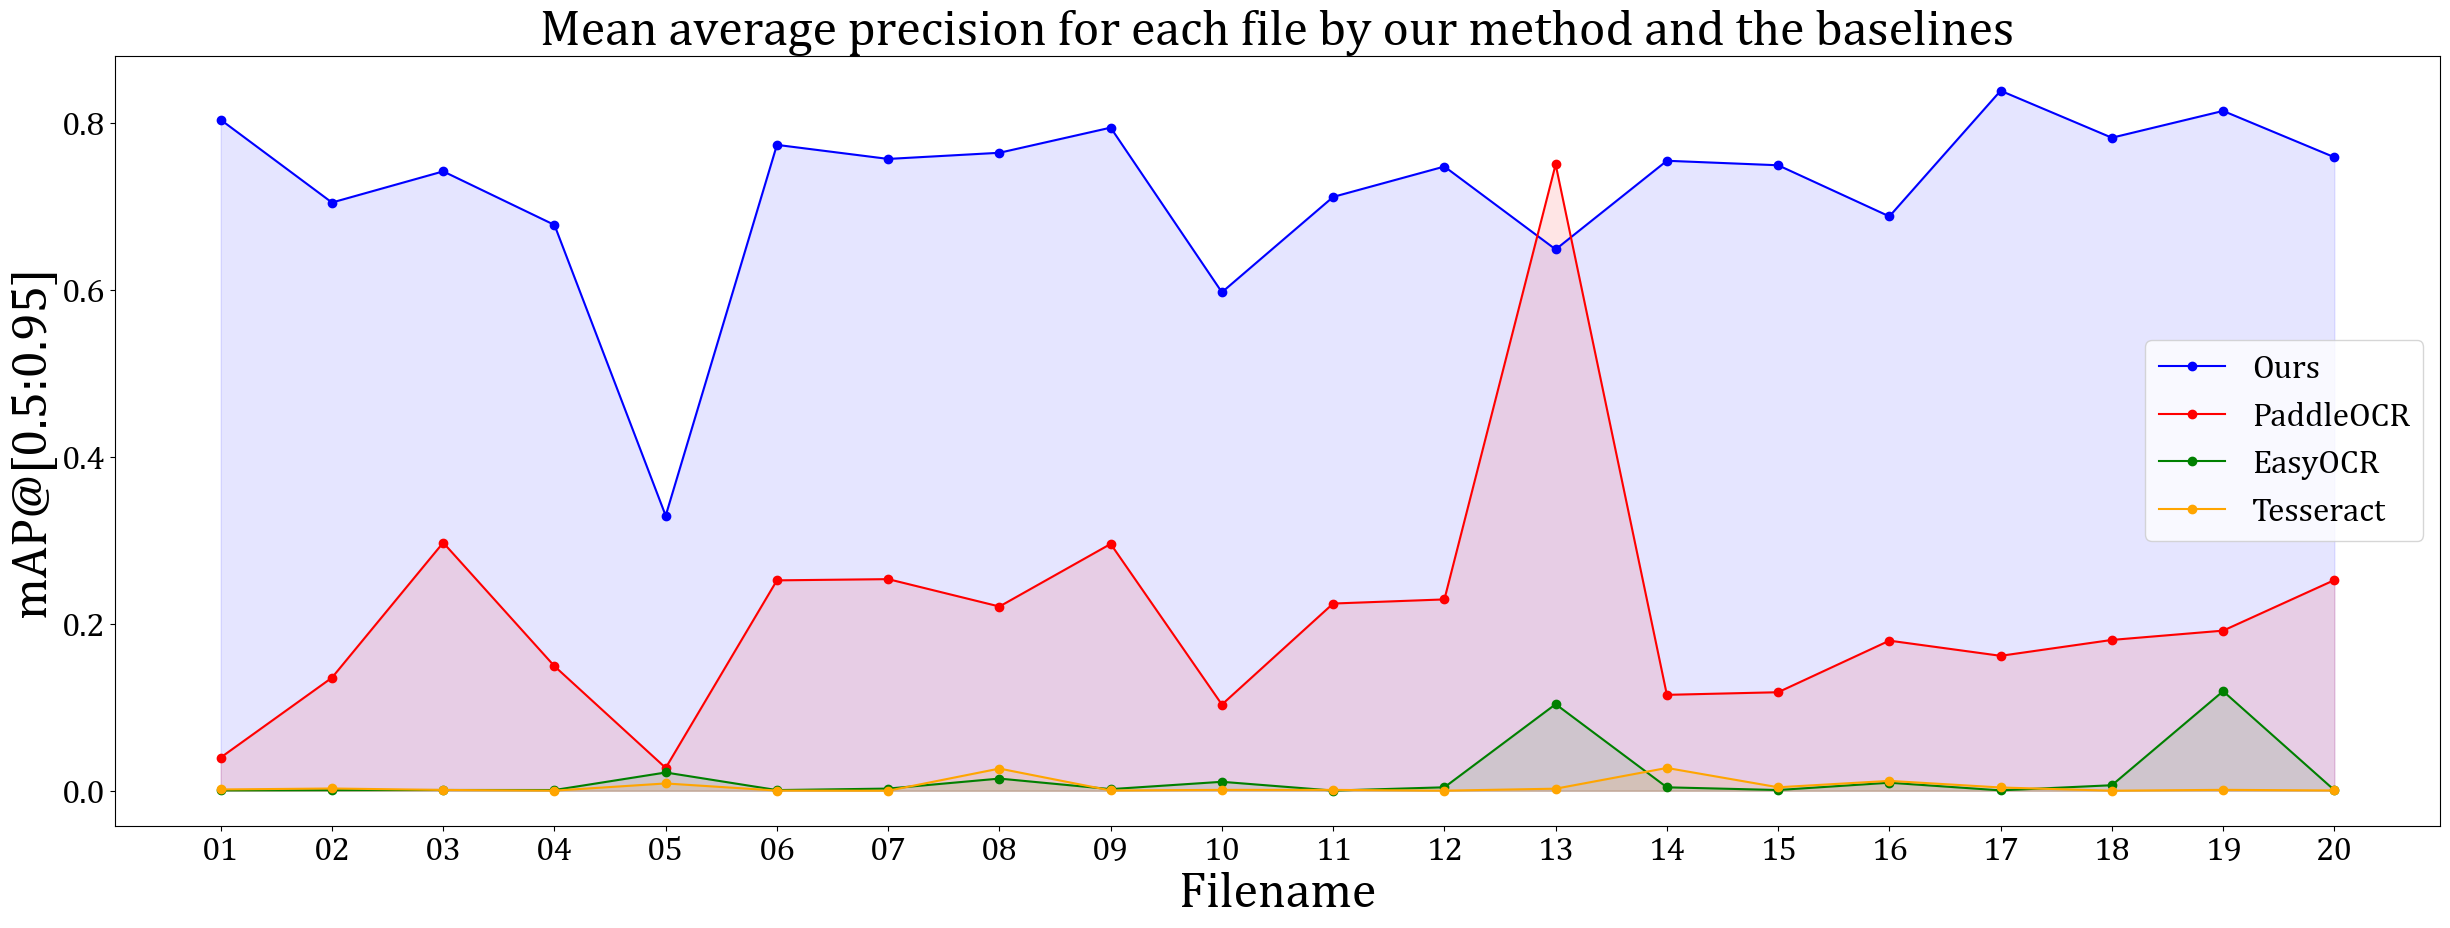
\includegraphics[width=\textwidth]{figures/comp_map2.png}
    \end{figure}
\end{frame}

\begin{frame}
    \begin{center}
        \Large{Comparison: Text Recognition}
    \end{center}
    \begin{itemize}
        \item The average CER is 12\% lower than AMP.
    \end{itemize}
    \begin{figure}
        \centering
        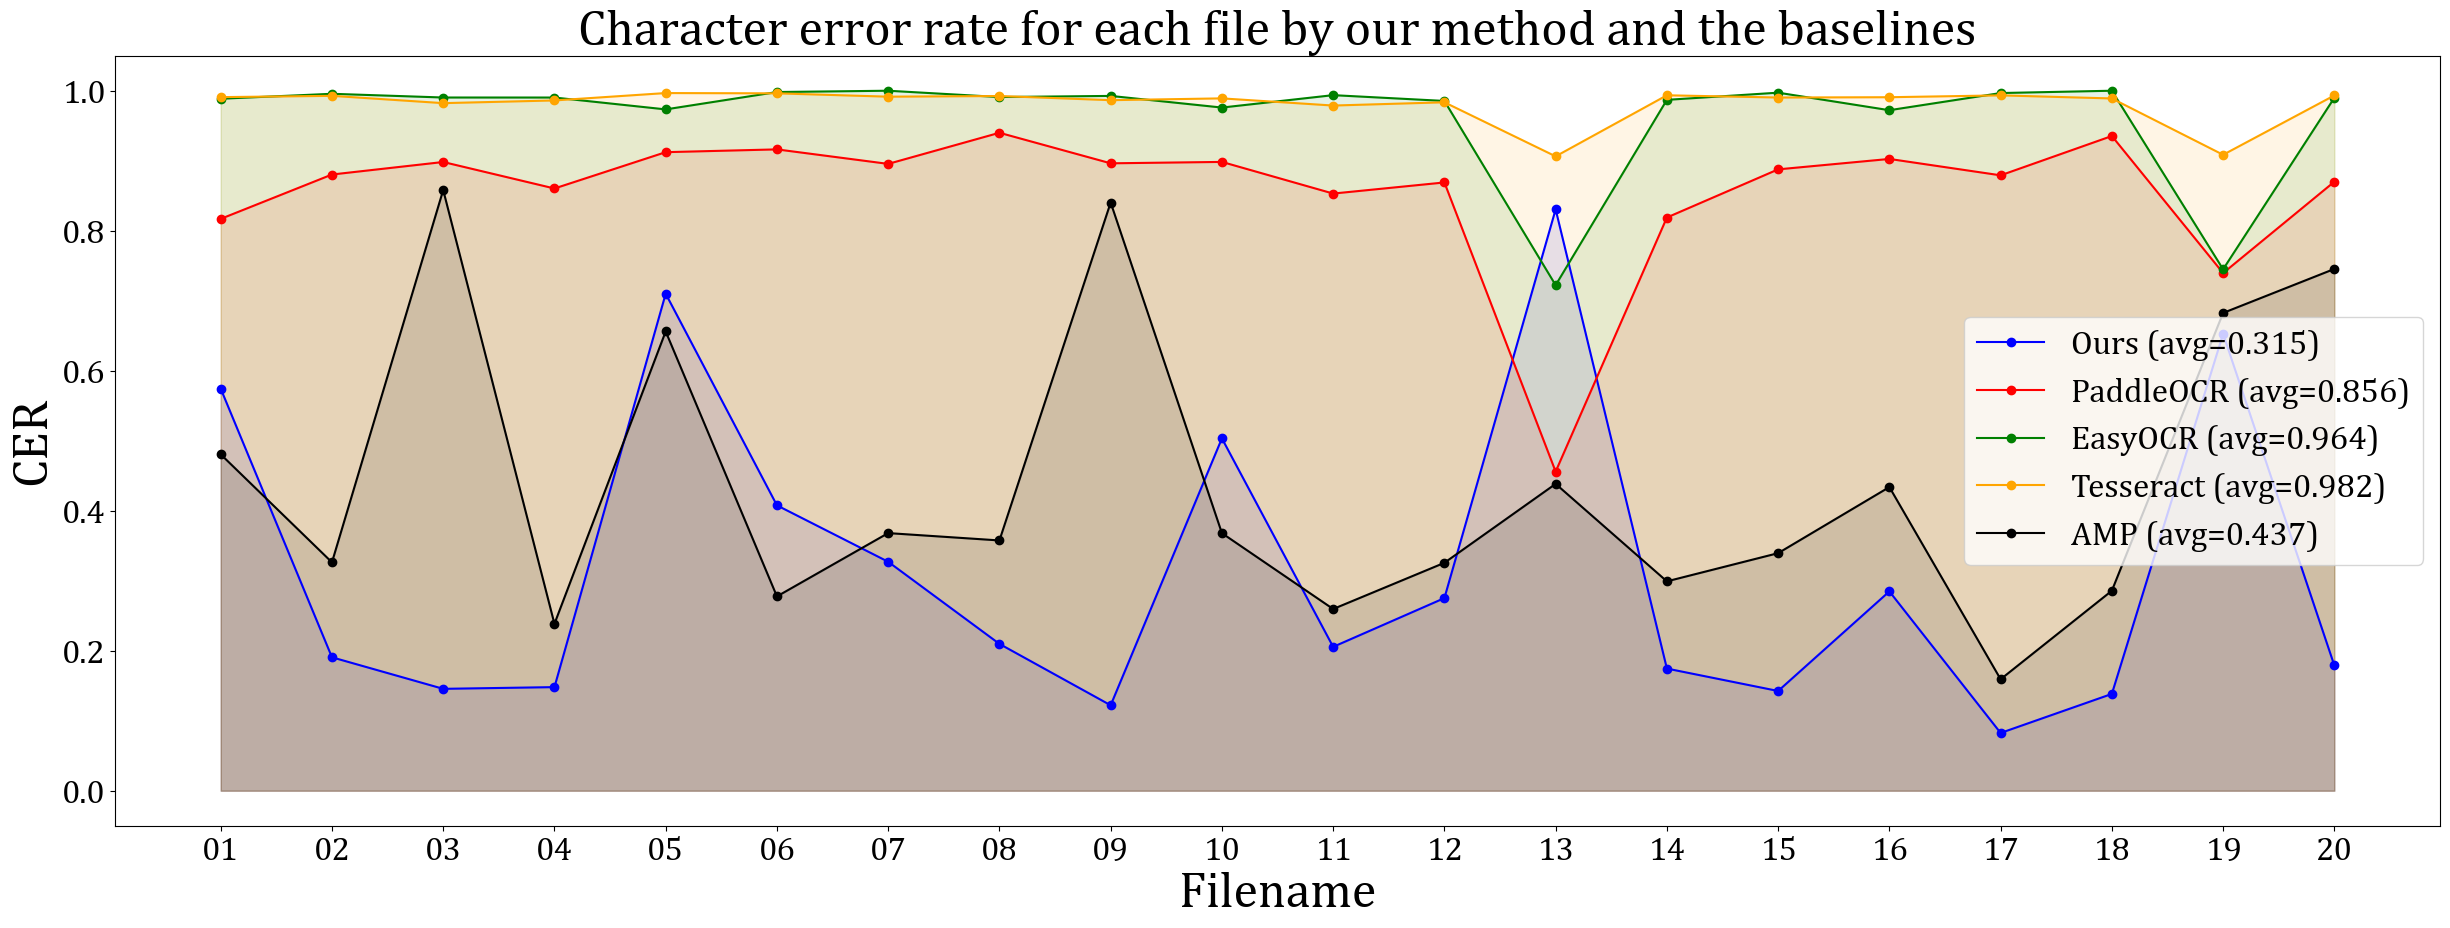
\includegraphics[width=\textwidth]{figures/comp_cer.png}
    \end{figure}
\end{frame}

\begin{frame}
    \begin{center}
        \Large{Comparison: Text Recognition}
    \end{center}
    \begin{itemize}
        \item The average BLEU-4 is 12\% higher than AMP.
    \end{itemize}
    \begin{figure}
        \centering
        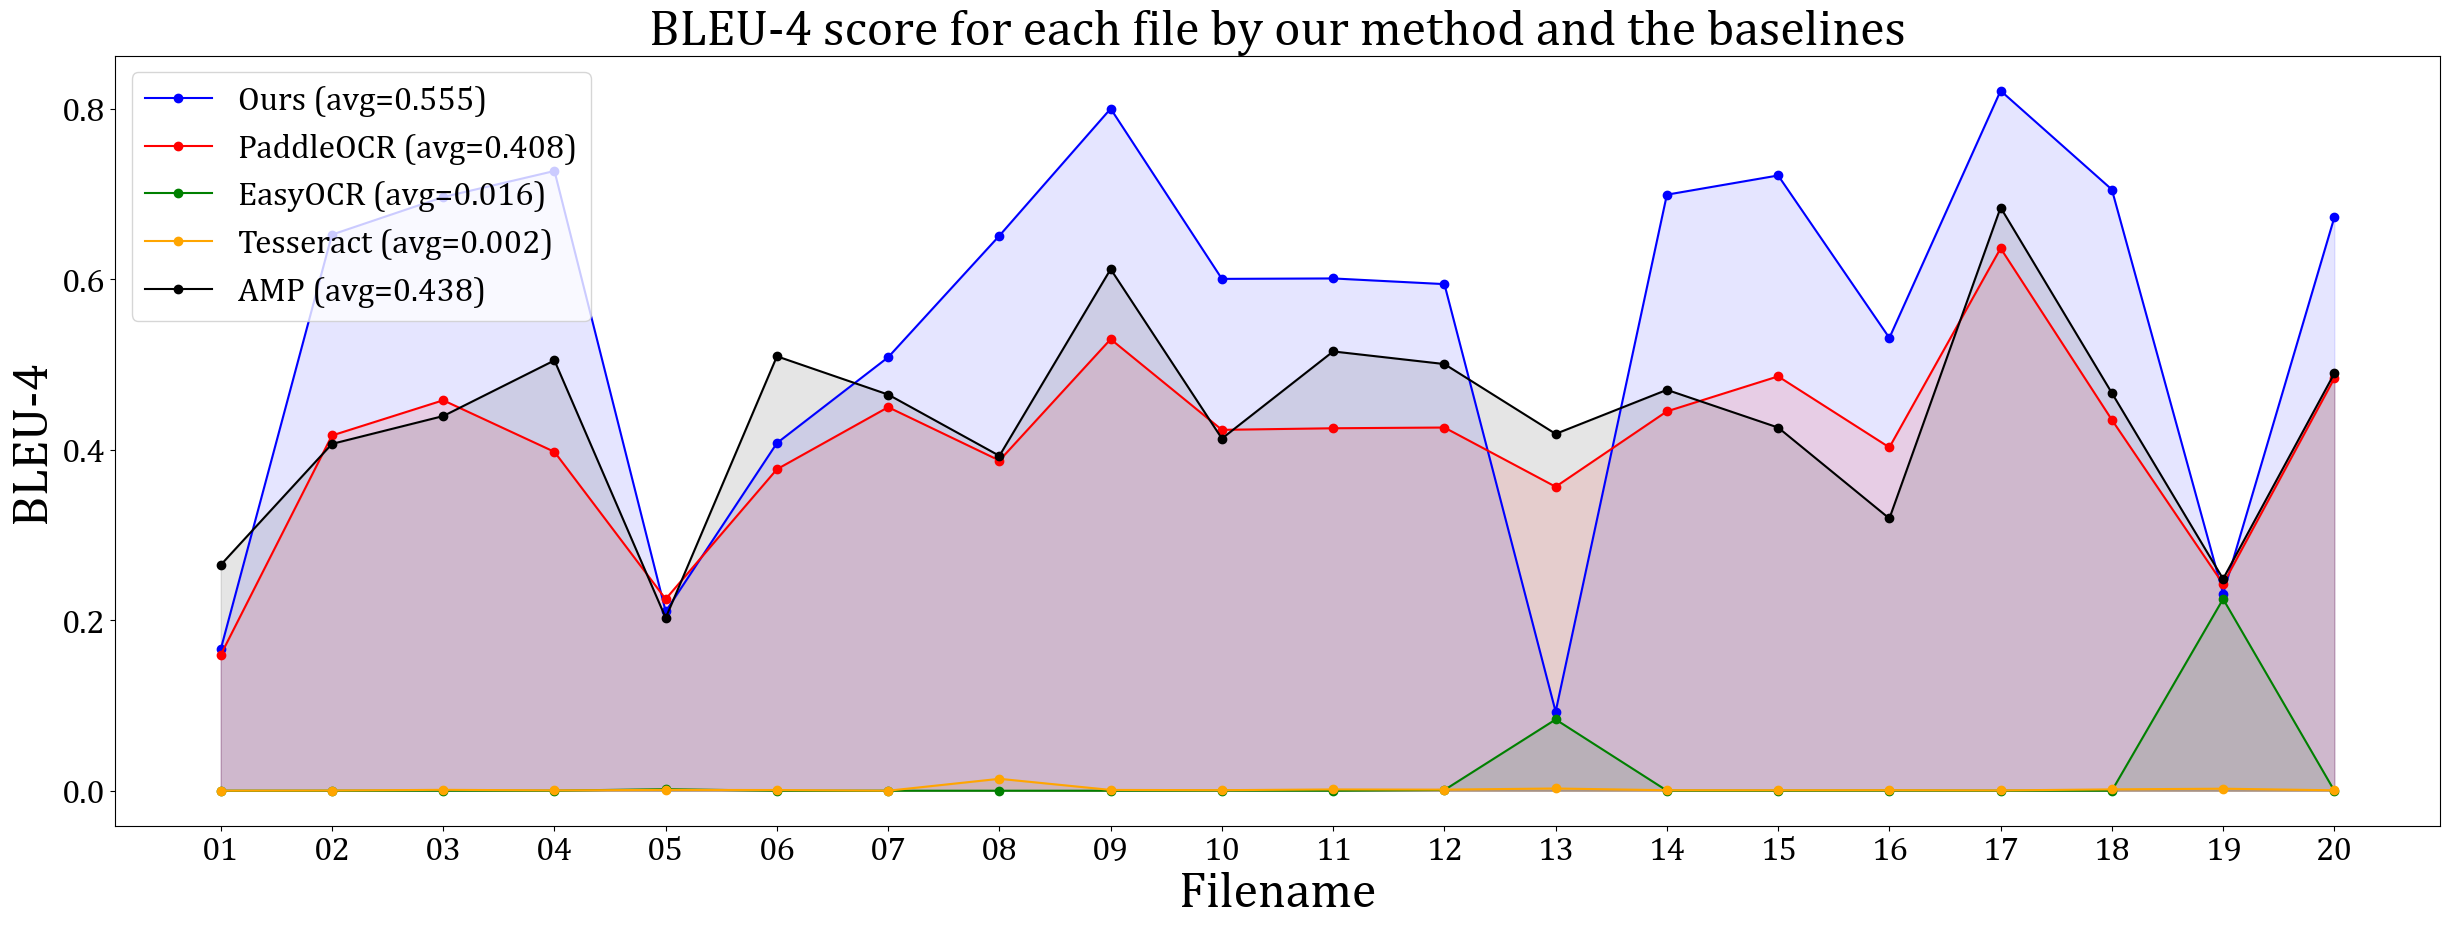
\includegraphics[width=\textwidth]{figures/comp_bleu.png}
    \end{figure}
\end{frame}

\begin{frame}
    \begin{center}
        \Large{Limitations}
    \end{center}
    \begin{itemize}
        \item Complex text layouts (a), large character spacing (b), horizontal text lines (b), and non-Chinese characters (c).
    \end{itemize}
    \begin{figure}[htbp]
        \centering
        \begin{subfigure}[b]{0.3\linewidth}
            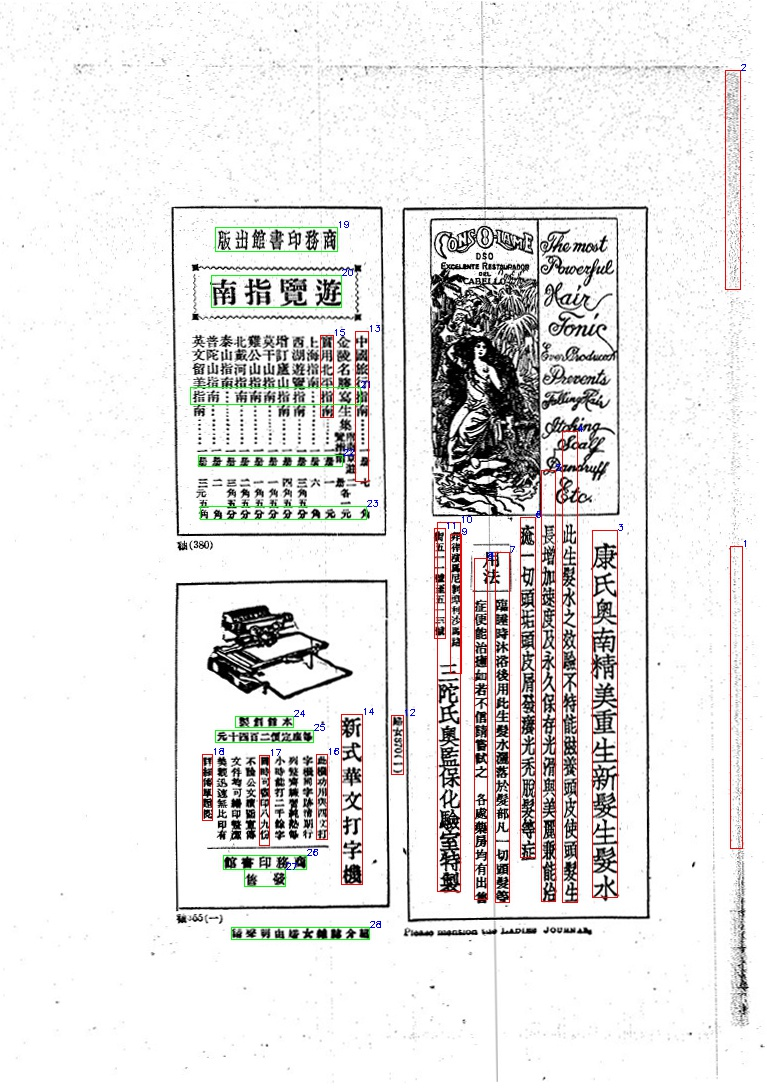
\includegraphics[height=1.35\linewidth]{./figures/samples/05.jpg}
            \caption{05}
            \label{fig:ours_05}
        \end{subfigure}
        \hfill
        \begin{subfigure}[b]{0.3\linewidth}
            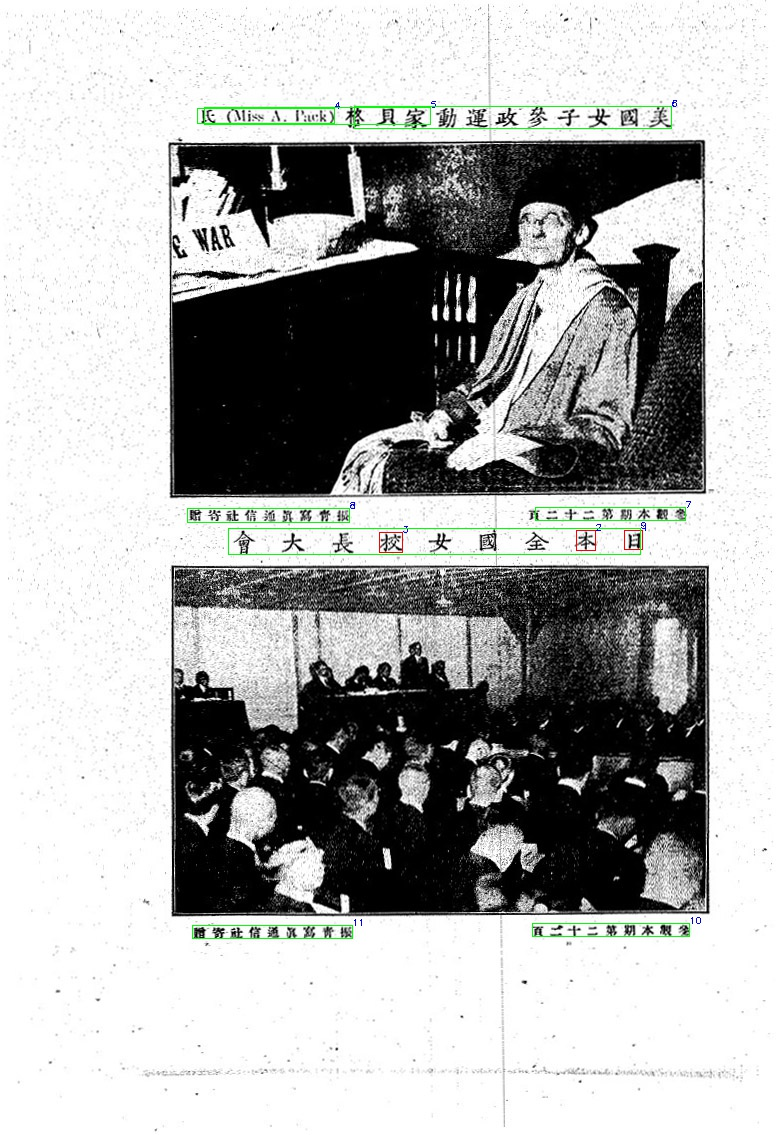
\includegraphics[height=1.35\linewidth]{./figures/samples/13.jpg}
            \caption{13}
            \label{fig:ours_13}
        \end{subfigure}
        \hfill
        \begin{subfigure}[b]{0.3\linewidth}
            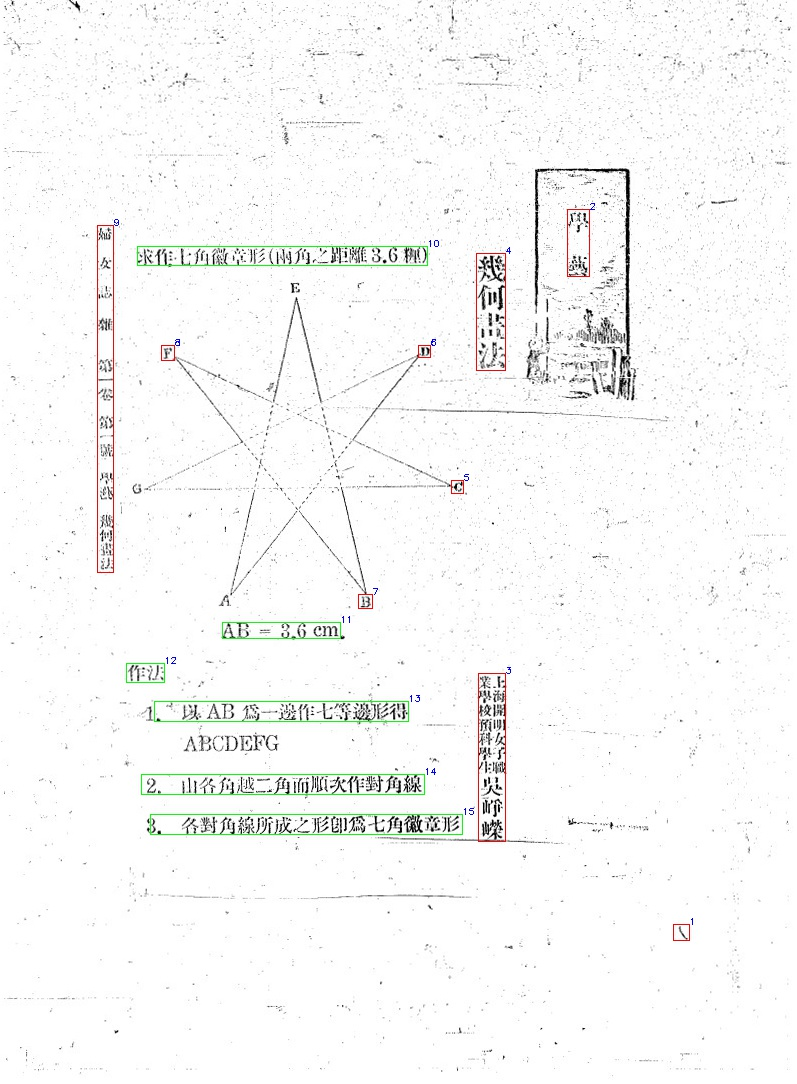
\includegraphics[height=1.35\linewidth]{./figures/samples/19.jpg}
            \caption{19}
            \label{fig:ours_19}
        \end{subfigure}
        \label{fig:challenging_cases}
    \end{figure}
\end{frame}

\begin{frame}
    \begin{center}
        \Large{Conclusion}
    \end{center}
    \begin{itemize}
        \item Developed an OCR system optimized for Funü Zazhi.
        \item Designed synthetic data to simulate Funü Zazhi images for training text detection and recognition models.
        \item Converted 36,101 images into text data, with about 30\% achieving CER of 0.15 and BLEU-4 of 0.73.
        \item Achieved superior performance compared to 4 SOTA OCR tools on the test dataset.
    \end{itemize}
\end{frame}

\begin{frame}
    \begin{center}
        \Large{Future Work}
    \end{center}
    \begin{itemize}
        \item Collect real annotated data for fine-tuning.
        \item Improve text ordering algorithms.
        \item Enhance synthetic data generation.
        \item Evaluate on relevant datasets.
        \item Extend to other historical documents.
        \item Deploy the system for public use.
    \end{itemize}
\end{frame}

\begin{frame}
    \begin{center}
        \Huge{Q\&A}
    \end{center}
\end{frame}

\begin{frame}
    \begin{center}
        \Huge{Thank you!}
    \end{center}
\end{frame}

\end{document}
